\documentclass[12pt]{report}

\usepackage[french]{babel}
\usepackage[utf8]{inputenc}%pour le é 
\usepackage[T1]{fontenc}
\usepackage{fancyhdr}%pour l'en-tete 
\usepackage{graphicx}%pour les images
\usepackage[margin=1in]{geometry}
\usepackage{cite}%pour bibliographie 
\usepackage{wrapfig} %pour figure a coté du texte
\frenchbsetup{StandardLists=true} % à inclure si on utilise \usepackage[french]{babel}
\usepackage{enumitem}
\usepackage{amssymb}
\usepackage[section]{placeins}
\usepackage{glossaries}


\usepackage{subcaption}
\setcounter{tocdepth}{3}
\setcounter{secnumdepth}{3}
%		Header		%		
\usepackage{fancyhdr}
\pagestyle{fancy}
\rhead{\thepage}
\lhead{\leftmark}

\usepackage{makeidx}
\makeindex

%subsubsubsection%

\makeglossaries
 
\newglossaryentry{MSA}
{
    name=MSA,
    description={Modern Standard Arabic. }
}

\newglossaryentry{CA}
{
    name=CA,
    description={Classical Arabic. }
}

\newglossaryentry{DA}
{
    name=DA,
    description={Dialectal Arabic. }
}

\input{Parts/commands.tex}


\begin{document}
\input{Parts/remerciements.tex}
\input{Parts/resume.tex}
\listoffigures  % table des figures



\tableofcontents
%\newpage
\chapter*{Introductions génerale}
La révolution numérique et technologique actuelle procure des changements importants dans des différents secteurs particulièrement le secteur industriel qui connaît une croissance et un développement exponentiel à tous les niveaux ce processus de changement technologique a débuté avec la révolution industrielle qui a connu un basculement très fort d’une société artisanal vers une industrie commerciale et industrielle voir l’émergence d’industrie virtuelle en adoptant de nouvelle techniques. Les tendances actuelles exigent aux entreprises manufacturières qu’elles soient flexibles, compétentes et réactives et qu’elles s’adaptent rapidement face aux perturbations externes telles que les fluctuations du marché et aux perturbations internes telles que l’indisponibilité de ressources. 

Ce concept de progression permet de passer d’une politique tout à fait alentour de produit à une économie client (la production ne concentre plus sur le produit, mais plutôt sur les exigences du client.  C'est pour cela les entreprises tente à faire des changements au niveau de leur chaîne logistique et de leur système productif par l’utilisation de nouvelles stratégies, actualisation de nouveau procédé de fabrication en appuyant sur l’écoute du client afin de rester compétitive dans un marché très concurrentiel.). La bonne gestion de la chaîne logistique permet aux entreprises industrielles et commerciales, de se positionner dans un marché très concurrentiel et répondre de manière efficiente aux différentes fluctuations. Ces exigences permettront aux entreprises de confronter plusieurs défis, tels que, la réduction des délais de fabrication et de livraison, diminution des prix, et cela sans pour autant affecter la qualité des produits et la qualité de service. Dans le but de répondre aux exigences actuelles, il est impératif de veiller sur l’amélioration continue des performances de l’entreprise qui s’élabore par une bonne gestion de toutes les opérations au sein des entreprises. En effet à l’heure actuelle digitale, sont au cours tous les phénomènes, la vision de l’amélioration continue est déjà bien engagée, et les industriels deviennent plus concurrentiels, plus productifs et misent sur les opportunités et les performances a adapté au sein de leur entreprise pour une meilleure réactivité et un meilleur rendement.

Cette dynamique sensible du marché, rehausse constamment les normes des industriels qui souhaitent accroître leur part de marché et satisfaire leurs clients. A cet égard, les erreurs et défauts de production de toutes causes confondues sont peu tolérés voir même intolérés chez certains producteurs en donnant une grande importance au contrôle de la qualité tout au long du processus. 

Pour répondre à ce contexte, les différents acteurs se tournent vers le développement des solutions innovantes facilitant les activités de production et le repérage des différents dysfonctionnements et des défauts de qualité. Le concept de l’industrie 4.0 se trouve au cœur de ces changements par la mobilisation des nouvelles technologies telles que les IOT (Internet Of Things), l’intelligence artificielle (IA) et le deep learning etc. 

L'intelligence artificielle a introduit plusieurs technologies dans l'industrie, évidemment dans le concept de qualité et de détection des défauts. L'IA à travers ses composants, notamment l'apprentissage profond, a donné naissance à des applications de vision artificielle spécialisées dans la détection de ces défauts de production.

La tendance dans ces applications est d'atteindre une précision de niveau humain ou mieux dans l'inspection de la qualité. Cela implique un minimum d'erreurs dans la production. Et donc une bonne réputation de l'entreprise sur le marché.
L'objectif de ce travail est de proposer une application de détection de non-conformité par apprentissage profond appliquée à un système de production alimentaire de nouilles référencé à la société JUMBO.

Le travail présenté dans ce mémoire se décompose en deux partie, la première abordera une recherche bibliographique sur la qualité et l’inspection de la qualité dans le contexte de l’industrie 4.0, suivant trois chapitres comme suit :
\begin{itemize}
    \item Un premier chapitre est  dédié  a présenté les notions de  contrôle de la qualité dans l’industrie 4.0  afin de  positionner  notre abordée dans le contexte de l’industrie 4.0.
    \item Un deuxième chapitre porte sur l’intelligence artificielle et ses composantes pour expliquer la science derrière les applications de l’industrie 4.0.
    \item Un troisième chapitre sur les systèmes de vision artificielle et le traitement d'images qui décrira tous les outils nécessaires pour construire une application de détection des défauts par vision artificielle.
\end{itemize}



La deuxième partie de ce travail concerne nos apports et contributions dans ce projet est décomposée également en deux chapitres comme suit : le quatrième chapitre sur le cadre méthodologique, et le cinquième  chapitre sur l’étude comparative et le choix du modèle.

Ce projet final est le résultat d'une tentative d'utiliser autant que possible les connaissances et les capacités que nous avons acquises au cours de notre programme éducatif. L'entreprise RMBtech Smart Automation, qui nous a accompagnés dans ce projet, nous a offert le cadre et l'environnement pratiques dans lesquels nous avons travaillé.

\part{Cadre contextuel et conceptuel}
%\chapter{Contrôle de la qualité dans l’industrie 4.0}
\section{Introduction}
Les anomalies au niveau du processus de production ont toujours été un défi pour l’industrie. Toute personne qui effectue une inspection visuelle répétitive peut se fatiguer, s'ennuyer ou être distraite. Comme les processus de production deviennent plus complexes, le risque d'erreurs humaines augmente ce qui peut entraîner des dégradations des produits finis engendrant des reprises coûteuses et fastidieuses pour le producteur. 

Ce qui a poussé les chercheurs à introduire L'industrie 4.0 qui désigne la transformation et la digitalisation continues des pratiques de production industrielles cela pour améliorer la productivité et la qualité de la production en éliminant les erreurs humaines via l'automatisation et l'utilisation des solutions logicielles d'analyse vidéo en obtenons des informations exploitables à partir des données de la chaîne logistique globale. Ces données peuvent non seulement être vérifiées et comparées en temps réel, mais aussi analysées dans le temps pour faciliter la prise de décision, la planification de la production et l'amélioration des processus.  

Ce que nous pouvons résumer dans ce chapitre, nous allons commencer par le concept de l'industrie et de la révolution industrielle. Nous passerons en revue les différentes techniques de l'industrie 4.0 et nous terminerons par le concept de qualité 4.0 qui relie l'industrie 4.0 au contrôle de la qualité. 
\section{Révolutions industrielles et évolution de l'industrie }
\subsection{Définition de l’industrie}
L'industrie est un terme polysémique recouvrant originellement la plupart des travaux humains. Il s'agit à présent de la production de biens grâce à la transformation des matières premières ou des matières ayant déjà subi une ou plusieurs transformations et de l'exploitation des sources d'énergie\cite{IndustrieWikipedia}.

\newpage
\subsection{Les quatre révolutions industrielles}
L'un des événements historiques les plus significatifs de la civilisation contemporaine a été la révolution industrielle. En fait, cette période cruciale de l'histoire a entraîné d'importants changements dans la civilisation, notamment sur le plan technologique, social et économique. Le concept d'emploi, les formes de production, les moyens de transport et la structure de la société et de l'économie ont tous subi des changements importants depuis la révolution industrielle\cite{AlloprofAideAux}. La figure ci-dessus montre un schéma explique les étapes de la révolution de l’industrie.

\begin{figure}[h]
    \centering
    \includegraphics[width=13cm]{assets/PartOne/Chapterone/Evolutiondel'industrie.png}
    \caption{Evolution de l'industrie}
    \label{Evolutiondel'industrie}
    \end{figure}

    Cette révolution a passé par quatre phases depuis milieu du XVIIIe siècle (1750) \cite{RevolutionsIndustriellesIndustrie}.
\begin{itemize}
    \item \textbf{Première révolution industrielle}  (industrie 1.0) : C'est la révolution qui s'est produite au XVIIIe siècle, et qui a pour pilier la machine à vapeur. L'objectif était la productivité de la production. 
 
    \item \textbf{Deuxième révolution industrielle} (industrie 2.0) : Cela s'est produit au 19ème siècle jusqu'en 1940 et était basé sur l'électricité. Comme cela s'est produit en même temps que la Première Guerre mondiale, on s'est inquiété du manque de matériel utilisé pour la production. Pour cette raison, la maintenance commence à être une préoccupation, et nous pouvons même dire que c'est ici que la maintenance préventive est née. 
     
    \item \textbf{Troisième révolution industrielle} (industrie 3.0) :  C'est la révolution des systèmes informatiques, qui s'est produit dans les années 70. Cette révolution n'a pas eu le souci de la productivité comme les deux autres, et c'est à ce moment-là que le système industriel « Just in Time a été créé, ce qui a pour résultat la réduction du temps et l'optimisation dans le secteur industriel. 
     
    \item \textbf{Quatrième révolution industrielle} (industrie 4.0) : fait référence à la transformation de l’industrie et des systèmes de production grâce à l’introduction des nouvelles technologies. Son but est de créer des usines intelligentes, qui puissent s’adapter plus facilement aux nécessités et aux processus de la production. Alors que l'industrie 4.0 reste un concept relativement nouveau, de nombreux experts et scientifiques parlent de l'industrie 4.1, qui vise le zéro défaut\cite{chengIndustryIntelligentManufacturing2021}. 
     
    \item \textbf{Cinquième révolution industrielle} (l'industrie 5.0) : cette approche conduira à un nouveau modèle de coopération et d'interaction entre les humains et les machines du contexte de l’ergonomie. Mais ce concept n'est pas vraiment fait l'objet d'un consensus, il reste une simple notion théorique jusqu'à présent.\cite{IndustrieVaInduire2018}
\end{itemize}


En 2012, l'Allemagne a proposé le terme de l'industrie 4.0 pour faire les premiers pas vers la prochaine révolution industrielle. La définition et les technologies de base de l'industrie 4.0 sont présentées ci-dessous.

\subsection{Définition de l’industrie 4.0}
Il est difficile de trouver une définition du concept « Industrie 4.0» qui fait consensus. La transdisciplinarité du concept, traduite par le vif intérêt accordé audit concept, conduit à l'émergence d'une diversité terminologique telle que 
\begin{itemize}
    \item industrie future
    \item industrie numérique
    \item industrie intelligente
    \item internet industriel
    \item transformation numérique
\end{itemize}
C'est ainsi qu'en 2013, BITCOM, l'association des télécommunications allemandes a trouvé plus de 100 définitions du concept de l'industrie 4.0. Cependant, afin de mieux cerner le sujet et limiter l'impact de la diversité des définitions, il est essentiel de ne citer que les définitions les plus importantes.

Par exemple, pour Schumacher \cite{schumacherMaturityModelAssessing2016} «Industrie 4.0 fait référence aux avancées technologiques récentes dans lesquelles Internet et les technologies associées (par exemple, les systèmes intégrés) servent de pivot pour intégrer des objets physiques, des acteurs humains, des machines intelligentes, des lignes de production et des processus dépassant les limites organisationnelles afin de former une nouvelle chaîne de valeur plus agile, intelligente et connectée».

Pour notre cas de recherche, nous prendrons la définition donnée par Pierre Cléroux, vice-président, Recherche et économiste en chef à la BDC, qui a défini ce terme comme suit : "à la base, l'industrie 4.0 consiste à surveiller et à contrôler vos machines et équipements en temps réel en installant des capteurs à chaque étape du processus de production".

\newpage
\subsection{Technologies 4.0}
Cette section vise à identifier les principaux groupes de technologies introduits par l'industrie 4.0. Nous avons utilisé une liste des différentes catégories qui désigne les principales technologies qui influencent ce développement industriel. Ces catégories sont :
\begin{itemize}
    \item Technologies relatives aux données.
    \item Technologies relatives à la communication.
    \item Technologies relatives au calcul et au traitement de données.
    
\end{itemize}
Ces catégories sont détaillées ci-dessous :

\subsubsection{Technologies relatives aux données}
\paragraph{La big data : }

Les données se considèrent comme étant de la matière première du 21ème siècle. En fait, la quantité de données dont disposent les entreprises semble presque doubler chaque année puisque, en 2020, plus de 50 milliards d'appareils seront connectés à l'échelle mondiale. La mégadonnées ou Big Data est non seulement une technologie, mais également un puissant outil pouvant fournir des informations, guider, inspirer et définir en profondeur la stratégie organisationnelle des campagnes.

Le traitement des données est conçu pour analyser, nettoyer, transformer et modéliser de variable source et format de données, permettant alors de créer des connaissances, du sens et des solutions pouvant servir pour prendre des décisions. Elle permet aussi de conférer aux données une dimension économique en faisant recours aux méthodes analytiques comme la corrélation, le regroupement, la régression ou l'analyse bayésienne qui est désormais importante.

Ainsi, les techniques associées aux mégadonnées aident alors à maximiser la qualité de la production, à augmenter l'efficacité, à optimiser la qualité des équipements et encore, à atteindre une productivité sans précédent.

\paragraph{La cyber sécurité :}

La cybersécurité assure une gestion de la data dans des conditions optimales et sécurisées. Elle permet la protection des systèmes d’informations et des données qui circulent contre ceux que l’on appelle les cybercriminels. Les compétences en informatique acquises par les personnes malveillantes sont des risques à ne pas prendre à la légère. De l’installation d’un antivirus jusqu’à la configuration de serveurs, ou encore le gardiennage des datas centers et des bureaux, la sécurité informatique impacte tous les métiers\cite{CybersecuriteDefinitionCybersecurite}.

Outre les cyberattaques, la cybersécurité permet la mise en place de processus auprès des collaborateurs pour l’instauration de bonnes pratiques. En effet, les erreurs humaines sont des sources réelles de fuites de données. La sensibilisation des équipes aux problématiques de phishing ou d’usurpation d’identité est une composante importante d’une politique de sécurité informatique.

Les entreprises ont besoin de processus de cybersécurité fiable et performant afin de travailler dans de bonnes conditions. La protection des données sensibles est essentielle pour garantir l’intégrité de chaque collaborateur, mais aussi des clients et des partenaires.

\newpage
\paragraph{Les capteurs intelligents}

Un capteur intelligent est un dispositif qui prend des données de l’environnement physique et utilise des ressources de calcul intégrées pour exécuter des fonctions prédéfinies lors de la détection d’une entrée spécifique, puis traiter les données avant de les transmettre.

Les capteurs intelligents permettent une collecte plus précise et automatisée des données environnementales avec moins de bruit parmi les informations enregistrées. Ces dispositifs sont utilisés pour les mécanismes de surveillance et de contrôle dans une grande variété d’environnements, notamment les smart grids, la reconnaissance des champs de bataille, l’exploration et un grand nombre d’applications scientifiques.

Le capteur intelligent est également un élément crucial et intégral de l’Internet des objets (IoT), l’environnement de plus en plus répandu dans lequel presque tout ce qui est imaginable peut être doté d’un identifiant unique (UID) et de la capacité de transmettre des données par internet ou un réseau similaire. Les capteurs intelligents sont notamment utilisés comme composants d’un réseau de capteurs et d’actionneurs sans fil (WSAN) dont les nœuds peuvent se compter par milliers, chacun d’entre eux étant connecté à un ou plusieurs autres capteurs et hubs ainsi qu’à des actionneurs individuels.

Les ressources de calcul sont généralement fournies par des microprocesseurs mobiles de faible puissance. Un capteur intelligent se compose au minimum d’un capteur, d’un microprocesseur et d’une technologie de communication quelconque. Les ressources de calcul doivent faire partie intégrante de la conception physique un capteur qui se contente d’envoyer ses données pour un traitement à distance n’est pas considéré comme un capteur intelligent\cite{CapteurIntelligent2020}.

\subsubsection{Technologies relatives à la communication}
\paragraph{Internet des objets (loT) :}
Internet est à l'origine un produit d'évolution progressive caractérisé tout d'abord par le Web 2.0 favorisant une communication à double sens et faisant référence à la possible interaction, collaboration et participation pouvant exister dans l'utilisation traditionnelle des réseaux sociaux, des blogs et autres. Ensuite, ledit Web 3.0 « sémantique » qui pour analyser, transformer et partager des informations standardisées, offre aux machines non seulement des informations compréhensibles et en ligne, mais leur permet aussi de naviguer sur les moteurs de recherche sans intervention humaine. Dès lors, ces technologies ont atteint un niveau avancé de développement qui a mené, aujourd'hui, à Internet des Objets. Celui-ci forme un réseau informatique interconnectant les objets, capteurs et des dispositifs autres que les ordinateurs. 

Tout en permettant audits dispositifs d'émettre, échanger et utiliser des données indépendamment de l'intervention humaine. L'internet des objets est ainsi une technologie permettant l'incorporation d'une capacité de communication auto-organisée et autonome aux différentes machines. L'interconnexion des objets physiques et des ressources numériques forme un réseau d'information qui facilite le contrôle de l'état des produits ou des systèmes et décentralise la prise de décision.

\newpage
\paragraph{Communication inter-machine (M2M)}
Le développement de la technologie de communication inter machines est dû à l'augmentation du nombre de systèmes et de machines autonomes. La technologie M2M est directement basée sur des protocoles et technologies de communication standard pour créer des réseaux de machines et de systèmes. Cette technologie peut faciliter l'échange direct entre les machines d'une grande flotte. En conséquence, le processus de production dans son ensemble, peut être reconfiguré pour réagir aux dangers rencontrés.

De plus dans les environnements de l'industrie 4.0, la technologie M2M est prête à remodeler divers aspects de fabrication, en particulier l'efficacité opérationnelle, le contrôle qualité, la prise de décision, les relations avec les clients, et les opportunités transactionnelles .Ainsi, l'accès à des actions en temps réel est nécessaire pour établir des organisations plus intelligentes et plus agiles, ce qui permet à la direction de mieux administrer les ressources, protéger les actifs spécifiques de l'entreprise, déployer des applications intelligentes pour élargir la portée et répondre rapidement aux exigences environnementales à évolution rapide. De plus, avec une bonne intelligence, livrée en temps réel et utilisée de manière appropriée, les services peuvent être proposés et adaptés aux clients de la meilleure façon possible.

\paragraph{Systèmes cyber physique}
À travers le temps, les mécanismes de traitement de l'information ont connu une évolution allant de grands ordinateurs centraux, passant par les ordinateurs personnels pour enfin arriver à des objets de calcul incorporés. La performance de ces mécanismes, manifestée dans l'accessibilité à internet, la capacité de communiquer, stocker et calculer les données, permet de contrôler, surveiller l'ensemble des objets, systèmes et processus. 

Ainsi, la communication et l'interconnexion des systèmes d'informations, réseaux, processus, sous-systèmes, objets internes et externes, clients et fournisseurs, définies ce qu'on appelle un Système Cyber Physique (CSP). Et en effet, le CSP fusionne non seulement les mondes physiques et virtuels, mais aussi dispose les objets d'une capacité de communiquer avec l'environnement, de reconfigurer ou participer à la reconfiguration en temps réel pour répondre aux besoins immédiats. Ce qui fait que les machines, dans l'industrie 4.0, forment une entité cyber-physique qui communique dans d'environnements réels et virtuels. Celle-ci rend le positionnement de la machine au sein de la chaîne de valeur plus flexible de sorte que le processus de production est adapté à la demande instantanée et ne subit plus de temps d'arrêt.

\paragraph{Les robots collaboratifs :} Durant la dernière révolution industrielle, les robots ont occupé une place importante au point de remplacer les travailleurs. Ainsi en 2004 la présence des robots multifonctionnels et polyvalents dans les usines européennes s'est considérablement développée et doublée. Récemment, la robotique a été développée pour devenir un outil indispensable dans tous les secteurs. Les robots industriels ont une grande flexibilité inhérente en raison de la polyvalence des outils, capteurs et autres périphériques.

Cependant, l'effort nécessaire pour programmer et configurer l'ensemble du système de robot, par exemple lors de l'introduction d'un produit nouveau ou modifié, est élevé et limite la flexibilité utilisée \cite{michniewiczCyberphysicalRoboticsAutomated2014}. C'est ainsi que les robots sont utilisés dans les industries pour favoriser la répétition des tâches prédéfinies nécessitant peu d'adaptation et de reconfiguration.

\subsubsection{Technologies relatives au calcul et traitement de données}
\paragraph{L’intelligence artificielle :}
Le terme "intelligence artificielle" inventé par John McCarthy est souvent abrégé en "IA" (ou "AI" en anglais, signifiant intelligence artificielle). L'un de ses créateurs, Marvin Lee Minsky, l'a défini comme la construction de programmes informatiques qui exécutent des tâches qui sont actuellement exécutées de manière plus satisfaisante par les humains car elles nécessitent un niveau élevé de processus mentaux tels que : l'apprentissage perceptif, l'organisation de la mémoire et le raisonnement critique.

Nous n'allons pas détailler ce concept car nous allons consacrer un chapitre entier qui parle de l'intelligence artificielle et de ces techniques de calculs et de traitement de données.

\paragraph{Cloud computing :}
Le cloud computing ou informatique en nuage est une infrastructure dans laquelle la puissance de calcul et le stockage sont gérés par des serveurs distants auxquels les usagers se connectent via une liaison Internet sécurisée. L'ordinateur de bureau ou portable, le téléphone mobile, la tablette tactile et autres objets connectés deviennent des points d'accès pour exécuter des applications ou consulter des données qui sont hébergées sur les serveurs.

De cette façon, l'entreprise peut recruter des services comme le stockage virtuel des données, pour les logiciels de gestion comme un ERP ou de sécurité du cloud, entre autres.
\begin{itemize}
    \item IaaS (infrastructure as a service) : C'est le premier service lancé par AWS qui donne à ses clients la possibilité d'utiliser des bases de données. Ainsi, au lieu d'acheter du matériel et de créer une salle de serveurs ou un centre de données, une PME pourrait louer des ordinateurs, du stockage et un réseau auprès d'un fournisseur de services en ligne.
    \item PaaS (Plateforme as a service) : C'est ainsi que Microsoft et d'autres ont réalisé que les développeurs avaient besoin non seulement d'une infrastructure, mais aussi d'un accès à des langages de développement de logiciels, à des bibliothèques et à des micro-services afin de créer des applications. Google fournit également le PaaS pour soutenir ses nombreuses applications domestiques.
    \item SaaS (Software as a service) : Le précurseur du cloud sous la forme d'applications web, comme Salesforce.com, lancé en 1999. Le SaaS est une nouvelle façon d'accéder à un logiciel. Au lieu d'accéder à un serveur privé local hébergeant une copie de l'application, les utilisateurs utilisaient un navigateur web pour accéder à une application partagée basée sur un serveur web. Comme le cas des ERP qu'ils sont devenus l'application généralisée de SaaS dans l'industrie.

\end{itemize}
\newpage
\paragraph{Puces d'accélération des réseaux de neurones (NPU) :}

Un Accélérateur d'IA pour accélérateur d'intelligence artificielle (ou NPU, anglais : Neural Processing Unit) est une catégorie de microprocesseur ou de systèmes de calculs conçu pour accélérer un réseau de neurones artificiels, accélérer des algorithmes de vision industrielle et d'apprentissage automatique pour la robotique, l'internet des objets et autres tâches de calculs-intensifs ou de contrôle de capteurs. Il s'agit souvent de conceptions multicœurs et se concentrant généralement sur l'arithmétique de faible-précision, des nouvelles architectures de flux de données ou de la capacité de calcul en mémoire.

\paragraph{La réalité augmentée (AR) :}

Est une version améliorée du monde physique réel qui est obtenue grâce à l'utilisation d'éléments visuels numériques, de sons ou d'autres stimuli sensoriels délivrés via la technologie. C'est une tendance croissante parmi les entreprises impliquées dans l'informatique mobile et les applications d'entreprise en particulier.

Au milieu de l'essor de la collecte et de l'analyse de données, l'un des principaux objectifs de la réalité augmentée est de mettre en évidence des caractéristiques spécifiques du monde physique, d'améliorer la compréhension de ces caractéristiques et d'en tirer des informations intelligentes et accessibles pouvant être appliquées à des applications du monde réel.

Ces mégadonnées peuvent contribuer à éclairer la prise de décision des entreprises et à mieux comprendre les habitudes de consommation des consommateurs en amont, comme elles peuvent jouer un rôle important en aval dans le cas des activités de marketing. En interne, la réalité augmentée fournit de nombreuses applications qui aident à l'industrialisation des produits tels que les simulateurs de systèmes de production.

\paragraph{Blockchain :}

La blockchain constitue une base de données distribuée sur un réseau de blocs, non plus contenus dans un seul épicentre. Ce réseau est souvent assimilé à un registre dans lequel sont enregistrées toutes les données ou transactions échangées/passées au sein de l'entreprise et de son environnement externe.

La blockchain est aujourd'hui surtout utilisée pour les transactions en monnaie virtuelle et n'est que rarement employée dans le secteur industriel. Il est logique de la voir appliquée dans le monde entièrement numérique d'aujourd'hui, où les transactions monétaires nécessitent une technologie fiable. Les experts de la transformation numérique, quant à eux, ont découvert des utilisations de la blockchain qui pourraient profiter au secteur informatique.

L'utilisation de "smart contracts" est envisageable. Il s'agit d'un type de contrat numérique qui se manifeste par des codes inscrits dans une blockchain, permettant le transfert automatisé d'actifs d'une entité à une autre (selon des règles de gestion prédéfinies). Ces smart contracts, en complément d'un ERP classique, permettent d'automatiser le processus de production (par exemple, commande sécurisée de matières premières automatiquement lorsque les stocks sont bas).

\newpage
\subsection{Prérequis de l'industrie 4.0}
Dans la littérature, plusieurs auteurs abordent les outils technologiques qui permettront la transformation vers l'industrie 4.0, tels que le Big Data ou l'Internet des objets. Cependant, peu d'auteurs se concentrent sur les prérequis à mettre en place pour réussir cette transformation numérique. Dans ce contexte, la littérature révèle deux écoles de pensée ; il y a l'approche technologique et l'approche des pratiques commerciales \cite{genestPrerequisitesImplementationIndustry2020}. 

Selon l'approche technologique, Pacchini expose les outils technologiques qui représentent l'industrie 4.0. Suite à ses recherches, l'auteur établit qu'il existe huit technologies le plus souvent associées à l'industrie 4.0 : L'Internet des objets, le Big Data, le Cloud computing, les Systèmes Cyber Physique, les robots collaboratifs, la fabrication additive, la réalité augmentée et l'intelligence artificielle. Afin de créer un modèle permettant d'évaluer le niveau de préparation des entreprises, l'auteur détermine que chaque technologie doit répondre à six pré requis préalables ; ces conditions doivent être remplies pour garantir la réussite de la mise en œuvre de la technologie. 

Pour chaque prérequis, une échelle à quatre niveaux est présentée pour établir le niveau de réalisation du prérequis. Par exemple, pour le niveau 0 : le pré requis n'est pas présent dans l'entreprise. Les scores associés aux pré requis permettent d'établir un résultat final sur le niveau de préparation numérique de l'entreprise, qu'il soit initial, primaire, intermédiaire, avancé ou prêt. Sur la base de ce résultat, l'entreprise peut s'orienter dans les prochaines étapes à franchir pour ensuite améliorer sa préparation numérique. Le tableau ci-dessous présente la liste de ces prérequis :

\newpage
%tablea%
tableau 

\newpage
%tablea%
tableau 
\newpage
D'autre part, plusieurs articles se concentrent davantage sur les actions à entreprendre et les pratiques commerciales à mettre en place avant même de penser à l'introduction réelle des technologies numériques. Selon Ranch, les conditions préalables à l'industrie 4.0 peuvent être représentées par 27 grands groupes : agilité, automatisation, connectivité, culture, conception pour la fabrication, numérisation, facilité d'utilisation, mise en œuvre, inspection, Lean, apprentissage automatique, personnalisation de masse, réseaux, personnes, planification et contrôle de la production, maintenance préventive et prédictive, contrôle à distance, gestion des ressources, sécurité, durabilité, suivi et traçage, transport, mise à niveau et réalité virtuelle. 

Chacun de ces groupes représente une liste d'actions nécessaires pour atteindre la préparation numérique.  Le total des exigences présentées dans ce document est de 65 actions. Par exemple, le groupe sur la production allégée comporte trois actions : l'entreprise doit réduire les activités sans valeur ajoutée dans la production et la logistique, produire à la demande et livrés juste à temps, et individualiser les produits le plus tard possible dans la chaîne de valeur.  Ces données ont été compilées à partir de consultations de PME lors d'ateliers en Europe, en Asie et aux États-Unis. À l'issue des ateliers, cinq conditions préalables ont été identifiées par les PME comme étant les plus importantes pour la transformation numérique. Le niveau d'importance des conditions a été associé à l'intérêt des PME participant aux ateliers.  Les cinq conditions préalables sont les suivantes : fabrication agile et personnalisation de masse, intégration de données en temps réel, numérisation et connectivité, mise en œuvre de technologies de fabrication avancées et d'automatisation, intégration de technologies faciles à utiliser avec un faible investissement et formation des employés à l'analyse des données intelligentes et à l'apprentissage automatique.

Toutes ces conditions préalables permettent aux PME de couvrir un ensemble de facteurs leur permettant d'être mieux préparées à la transformation vers l'industrie 4.0. Malgré le fait que les PME soient connues pour être flexibles et réactives aux besoins de leurs clients, il est essentiel pour les PME de compenser leur manque d'agilité et de connaissances en matière de fabrication, en améliorant leur expertise technologique, pour ensuite assurer le succès de la transformation.

\subsection{Contraintes à l'application de l'industrie 4.0
}
Si nous prenons en compte les contraintes des perceptions théoriques de base de l'industrie 4.0. Comme présenté précédemment, les principaux concepts autour de ce sujet sont les systèmes cyber-physiques (CPS), l'Internet des objets (IoT), et l'intelligence artificielle (AI). Par conséquent, nous formalisons les contraintes en combinant trois sources principales : Les principales contraintes des CPS, les principales exigences de l'IoT et les principes de l'intelligence artificielle.

En premier lieu, nous évaluons les systèmes cyber-physiques. Imposent que ces systèmes doivent rester entièrement opérationnels pendant le temps d'exécution de la tâche. Cette contrainte crée un besoin de protocoles de sécurité logicielle pour respecter les exigences de temps réel soft et hard. En outre, cela exige la robustesse et la fiabilité du matériel, qui est une contrainte de base des systèmes intégrés. Ces contraintes représentent un aspect de fiabilité dans les données produites, qui dépendent du matériel et du logiciel. 

Nous analysons également les principales contraintes de l'Internet des objets. L'objectif de l'Internet des objets est l'omniprésence de dispositifs décentralisés basés sur un réseau. Comme l'information est la valeur la plus importante, la capacité de communication du réseau est la principale contrainte du développement des applications de l'IoT. Nous affirmons que les réseaux de capteurs sans fil constituent la principale base théorique des applications de l'IoT. Ces applications nous apprennent que ces contraintes de réseau affectent la fiabilité des données.

Cependant, si l'on parle d'intelligence artificielle et de traitement des données, la qualité de ces données et l'industrialisation de leur traitement doivent également être mieux maîtrisées. Enfin, il n'est pas facile de mettre en place des processus d'intelligence artificielle sur un site industriel si l'on ne s'assure pas la qualité des données et de la précision des algorithmes de traitement.

Par conséquent, nous présentons trois contraintes les plus importantes dans la conception des applications de l'industrie 4.0 :

\begin{itemize}
    \item \textbf{La fiabilité du logiciel et du matériel :} En tant que CPS, l'application doit présenter des éléments matériels et logiciels fiables pour fournir l'environnement nécessaire au développement de la proposition.
    \item \textbf{Mise en réseau et communication :} En tant qu'application IoT, les dispositifs doivent fournir des services avec des contraintes de qualité minimales pour permettre des applications pleinement opérationnelles dans le contexte de l'industrie 4.0 avec une fiabilité des données.
    \item \textbf{La précision des algorithmes :} Il faut assurer la précision d’algorithmes utilisés pour le calcul et le traitement de ces données.

 
\end{itemize}

\section{La qualité 4.0}
La qualité est largement mise en œuvre par les entreprises et constitue un concept important dans les processus industriels, car elle représente un avantage concurrentiel. Aujourd'hui, il est presque obligatoire de suivre des normes de qualité pour mettre un produit sur le marché. Cependant, face aux nouveaux paradigmes de production, comme l'industrie 4.0, des questions se posent sur la manière dont les processus de gestion de la qualité pourraient bénéficier et s'adapter à l'ère des technologies numériques. Pour ce faire, dans cette section, nous commencerons par définir le concept de qualité et de systèmes de contrôle de la qualité de manière générale, puis nous ferons le lien entre les pratiques de qualité et les technologies de l'industrie 4.0 en introduisant la notion de qualité 4.0 qui donnera naissance au concept de systèmes intelligents de contrôle de la qualité.

\subsection{Définition de la qualité}
La qualité est un terme beaucoup plus compliqué qu'il n'y paraît.  Les définitions des dictionnaires sont généralement insuffisantes pour aider un professionnel de la qualité à comprendre le concept.  Il semble que chaque expert en qualité définisse la qualité d'une manière quelque peu différente. Parmi eux,ils ont défini la qualité par des normes internationales comme l’ISO 9001.

L’organisation internationale de normalisation (ISO) \cite{ISOOrganisationInternationale}, elle-même, présente une définition sur la qualité qui dit : « c’est l’ensemble des propriétés et caractéristiques d’un produit, processus ou service qui lui confèrent son aptitude à satisfaire les besoins exprimés ou implicites ».

Pour James TEBOUL, « c’est d’abord la conformité aux spécifications. C’est aussi la réponse ajustée à l’utilisation recherchée, au moment de l’achat et à long terme". Dans le cadre de ce mémoire nous allons prendre cette définition comme définition principale car elle s'intéresse à la conformité du produit \cite{ControleQualiteDefinition}.

Une définition de la conformité qui a été introduite par et qui dit : “Le produit est conforme lorsqu'il passe l’intégralité des tests de qualité avec succès et il peut passer à l’étape suivante. (Assemblage, commercialisation, etc.), alors qu’un produit est non-conforme lorsqu' il ne respecte pas une exigence. Cela passe principalement par la détection de la cause racine, puis on s’intéresse à la non-conformité pour voir si le produit est retouchable ou pas”. Pour avoir testé si le produit répond ou non aux exigences, l'entreprise a besoin d'une fonction de contrôle de la qualité. Nous allons définir le concept de contrôle de la qualité dans le point suivant.

\subsection{Evolution de la qualité}
Comme nous l'avons dit précédemment, l'évolution de l'industrie a influencé la qualité, le tableau ci-dessous explique l'évolution de la qualité en parallèle avec la révolution industrielle.
%Tab%
\newpage
tableau 
\newpage
tableau 
\newpage

\subsection{Définition de la qualité 4.0}
La qualité 4.0 est la quatrième vague du mouvement de la qualité. Cette philosophie qualité est construite sur les fondements statistiques et managériaux des philosophies précédentes. Elle exploite le Big Data industriel, l'Internet industriel des objets et l'intelligence artificielle pour résoudre une toute nouvelle gamme de problèmes d'ingénierie insolubles. La qualité 4.0 est fondée sur un nouveau paradigme basé sur l'apprentissage automatique, l’intelligence artificielle, la collecte et l'analyse de données en temps réel, pour permettre de prendre des décisions intelligentes \cite{escobarQualityReviewBig2021}.

La qualité 4.0 passe certainement par la digitalisation du contrôle qualité. Cette digitalisation des infrastructures qualité, des processus et des individus est plus importante à prendre en compte. Cette approche de la qualité peut remplacer les approches traditionnelles et améliorer les processus actuels. Les fabricants doivent utiliser le système de contrôle qualité 4.0 (ou systèmes de contrôle qualité intelligents) pour évaluer leur statut actuel et déterminer les ajustements nécessaires pour progresser dans le futur en matière de qualité. La connectivité de ces systèmes est transformée par un ensemble de capteurs embarqués peu coûteux qui fournissent aux individus connectés, aux biens et aux dispositifs et processus de pointe un retour d'information en temps réel \cite{javaidSignificanceQualityComprehensive2021}.

Les produits connectés peuvent fournir des avis sur le succès de leur cycle de vie. Cela relie efficacement les équipements critiques aux ordinateurs de périphérie câblés. Les capteurs Edge et puce spécialisées analysent également le système et prennent des décisions prédictives/prescriptives. Cet aspect de connectivité Qualité 4.0 permet de réduire globalement le processus de prise de décision en fournissant des données ouvertes et une analyse solide. La connectivité, les données et l'analyse ont été profondément transformées et développées en tant que source influente de créativité et d'assurance qualité.

\subsection{Le Contrôle de la qualité}
Selon Claude Laporte Le contrôle de la qualité est une opération destinée à déterminer, avec des moyens appropriés, si le produit (y compris, services, documents, code source) contrôlé est conforme ou non à ses spécifications ou exigences préétablies et incluant une décision d'acceptation, de rejet ou de retouche \cite{aprilAssuranceQualiteLogicielle2011b}.

Cependant, pour effectuer un contrôle sur un produit, il est nécessaire de déterminer ses caractéristiques et de choisir les limites dans lesquelles le produit est conforme. Ces limites doivent être connues par le contrôleur qui effectue le contrôle, qu'il s'agisse d'un être humain ou d'un système automatisé.

\subsection{Les enjeux de contrôle de la qualité}
L'importance du contrôle de la qualité va de la bonne image, l'augmentation des volumes de ventes et de la compétitivité, la bonne réputation, la fidélité des clients, pour n'en citer que quelques-uns. La concurrence mondiale. Pour cela on peut dire qu’un mauvais contrôle de qualité va influencer négativement sur l’entreprise.

Ainsi, le contrôle de la qualité n'est pas un simple outil de surveillance des entreprises, mais doit plutôt être considéré comme un mécanisme permettant d'anticiper les risques produits par la non-conformité des produits. Tels que le risque de réputation et nous pouvons citer ici le cas des chocolats Kinder, produits par le groupe alimentaire italien Ferrero, qui sont soupçonnés d'être à l'origine d'une épidémie de salmonellose en Europe, principalement chez les jeunes enfants. Ces risques peuvent se transformer en risques juridiques si les clients portent plainte auprès de la justice. Ces défis impliquent pour l'entreprise d'améliorer les activités de contrôle pour bien maîtriser les exigences du marché afin de garder la bonne image et de gagner la fidélité des clients.

\subsection{Systèmes de contrôle qualité intelligents}
Le concept de systèmes de contrôle de qualité intelligents (SCQI) est fondé sur le principe que dans la production intelligente, le contrôle de la qualité (CQ) est piloté par l'infusion de Big Data Analytics, de l'intelligence artificielle (AI), Systèmes Cyber-Physiques (CPS), Robotique et intensité des interactions Homme-Machine (H2M). Le concept remplace les systèmes de CQ traditionnels dans les processus de fabrication, car l'automatisation prend en charge la plupart des opérations ou des tâches qui étaient des tâches de routine effectuées par l'homme.

Le contrôle qualité intelligent est principalement exécuté pour gérer physiquement diverses machines ou outils intelligents. Ces technologies sont capables de communiquer à la fois avec les produits (produits intelligents) et leurs environnements. Ces gadgets fonctionnent de manière autonome pour créer une communication transparente entre eux. à travers des capteurs installés, et des techniques de simulation et d'intelligence artificielle aident à la conception et à la mise en œuvre d'un modèle de Machine Learning qui peut diagnostiquer et prédire tout défaut de qualité sur un produit. 

En résulte ces systèmes donnent une solution rentable de surveillance du processus de production pour améliorer la qualité des produits basés sur les technologies de l'industrie 4.0. La figure suivante décrit les systèmes de contrôle qualité intelligentes dans le cadre de l’industrie 4.0 :

\begin{figure}[h]
    \centering
    \includegraphics[width=6cm]{assets/PartOne/Chapterone/lesystèmesdecontrôlequalitéintelligentesdanslecadredel’industrie4.0.png}
    \caption{les systèmes de contrôle qualité intelligentes dans le cadre de l’industrie 4.0}
    \label{systemecontrolequalité}
    \end{figure}

\subsection{Les avantages des systèmes de contrôle qualité intelligents}
La qualité étant devenue une priorité pour les entreprises, de nouvelles approches sont désormais disponibles pour résoudre la complexité du contrôle de la qualité et éliminer les risques associés à cette fonction. La qualité 4.0 fait partie des nombreux développements qui donnent naissance aux industries du futur, qui ont amélioré numériquement les structures et les processus des usines afin d'accroître la productivité et la flexibilité tout au long de la chaîne logistique.

Cette approche de contrôle qualité intelligent offre quelques avantages majeurs aux entreprises qui les mettent en œuvre à grande échelle. Ces avantages sont résumés comme suit :

\begin{itemize}
    \item \textbf{Time to market} pour développer, produire et commercialiser de nouveaux produits et services, nécessitant une capacité d'innovation plus élevée et plus rapide. Cela est dû aux technologies de pointe telles que la fabrication additive, l'Internet des objets (IoT), la réalité augmentée et la réalité virtuelle. Ceux-ci ont éliminé les déchets qui étaient autrefois associés aux erreurs humaines, créant ainsi une production allégée de produits compétitifs à l'échelle mondiale. La réalité augmentée (AR) aide à réduire les défauts, les retouches et les inspections redondantes en offrant des informations intuitives et en combinant l'intelligence et la flexibilité de l'opérateur avec des systèmes anti-erreurs pour augmenter l'efficacité des étapes de travail manuelles, tout en améliorant la qualité du travail.
    \item \textbf{Une personnalisation} accrue pour satisfaire les demandes individuelles des consommateurs, sur un marché d'acheteurs et non plus de vendeurs, conduisant à une plus grande individualisation des produits ; ce qui signifie que les produits n'auront peut-être pas besoin d'être produits en masse comme auparavant, car les fabricants pourront produire de très petites séries (un seul produit si nécessaire). Cette technologie permet une configuration rapide des machines et du processus de production, ainsi que leur adaptation aux besoins des clients.
    \item \textbf{Une flexibilité} plus élevée avec des processus de production plus rapides et plus polyvalents capables de produire de plus petites quantités de lots avec une qualité élevée et de manière rentable.
    \item \textbf{Une précision} améliorée à une vitesse impossible avec des travailleurs humains, ces systèmes peuvent également être beaucoup plus rentables une fois qu'ils sont en place.
\end{itemize}
\newpage
\section{Conclusion}
Dans ce chapitre nous avons abordé le concept de la qualité dans le contexte d’industrie 4.0 et expliqué les technologies de pointe qui servent à appliquer des systèmes intelligents pour la détection de défauts et l'amélioration de la qualité.

L’intelligence artificielle est en train de dominer ce paradigme. Tous les niveaux et tous les secteurs de l’industrie sont en train d’être bouleversés par les technologies et les composantes de cette nouvelle discipline .

Dans le prochain chapitre nous allons détailler la science derrière le concept de l’intelligence artificielle et ces technologies de tendances.







\chapter{L’intelligence artificielle et ses composantes}
\section{Introduction}
L’industrie représente l’un des terreaux les plus fertiles pour l’intelligence artificielle, vue  l’amélioration de la compétitivité qu'apporte l’intelligence artificielle à l’industrie. En lui offrant plusieurs avantages particulièrement  . l’entreprise peut organiser sa chaîne logistique, maîtriser  les données et les flux, facilite l’analyse des paramètres qui influencent la performance d’une ligne de production,et, permettent de faire des propositions d’optimisation des procédés de production. 

Autre atout de l’intelligence artificielle descriptive est qu’elle permet de distinguer quelles sont les tâches pouvant être améliorées, et les autres. Intégrée aux machines et logiciels de planification, elle identifie les tâches répétitives à faible valeur ajoutée qui peuvent être automatisées et donc prises en charge par des systèmes intelligents. 

Dans la suite de ce chapitre, nous allons définir l'intelligence artificielle et toutes les notions incluses dans ce vaste concept, nous donnerons des explications mathématiques et informatiques dans des points critiques tels que le Deep Learning qui est une sous-famille de Machine Learning qui est lui-même inclus dans l'IA, la figure suivante illustre le positionnement des mots clés dans ce chapitre


\begin{figure}[h]
    \centering
    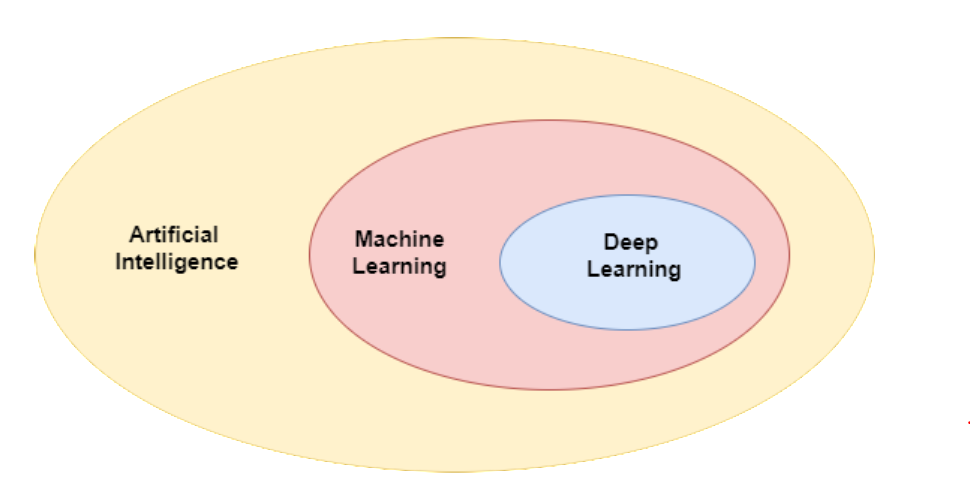
\includegraphics[width=10cm]{assets/PartOne/Chaptertwo/relationentreintelligenceartificielleetmachinelearningetdeeplearning.png}
    \caption{La relation entre l'intelligence artificielle, machine learning et deep learning}
    \label{relationentreintelligenceartificielleetmachinelearningetdeeplearning}
    \end{figure}

\newpage

\section{Intelligence artificielle}
\subsection{Définitions de l’intelligence artificielle}
La définition de l'intelligence artificielle a traversé de nombreuses définitions au fil des ans, et à ce jour il n'y a pas de définition officielle pour ce concept. Par exemple Asa B.Simmons et Steven G. Chappell \cite{simmonsArtificialIntelligencedefinitionPractice1988} ont défini le terme "intelligence artificielle" comme le comportement d'une machine qui, si un humain se comporte de la même manière, alors cette machine est considérée comme intelligente. Il est difficile d'étendre cette définition car la définition des facteurs qui décrivent l'intelligence humaine n'est pas claire.

Il existe une autre définition qui rend compte de la nature du travail effectué dans le domaine technologique. Elle a été proposée par E. Rich \cite{richArtificialIntelligenceHumanities1985} et se lit comme suit : ”L'intelligence artificielle est l'étude qui consiste à faire aux ordinateurs des choses que, pour l'instant, les humains font mieux.” Cette définition semble simple, mais critique en même temps, car il peut y avoir actuellement des machines qui surpassent les humains, par exemple, les systèmes prédictifs qui peuvent nous donner des résultats auxquels les gens ne pensent pas à travers les calculs complexes qu'ils effectuent.

Donc, comme nous l'avons déjà dit “L’intelligence artificielle” (IA) est une notion paradoxale car, comme le souligne Yoshua Bengio, on ne rend pas l’ordinateur plus intelligent mais on le rend au contraire moins stupide. Et on peut dire que L’IA est à la fois une discipline de recherche et une matière, à l’instar des mathématiques ou de la physique, utilisée dans de nombreuses autres disciplines de recherche, comme la médecine\cite{WillMachinesEliminate}.

Aujourd'hui plus que jamais, comprendre ce qu'est l'IA, ce qu'elle fait, ce qu'elle fera sûrement et ce qu'elle ne fera certainement jamais est un moyen ingénieux de comprendre et d'anticiper, même partiellement, le champ des possibles, et donc de s'y préparer, en tirant tous les bénéfices tout en écartant les éventuelles menaces.

Pour cela et en termes de définition simple, On peut définir l’IA comme l'intelligence artificielle est la capacité d'une machine ou d'un dispositif informatique à imiter l'intelligence humaine (processus cognitif), à acquérir des expériences, à s'adapter aux dernières informations et à réaliser des activités semblables à celles des humains\cite{klagesPatchBasedGenerative2019}.

\subsection{Typologie de l’intelligence artificielle}
Selon \cite{QuEstceQuea} l’IA peut être classée comme faible ou forte. L’IA faible, ou IA étroite, est un système d’intelligence artificielle conçu et entraîné pour une tâche particulière. Ainsi, les assistants personnels virtuels comme Siri d’Apple, sont une forme d’IA faible. Quant à l’IA forte, ou intelligence générale artificielle, elle dispose de capacités cognitives humaines.

\subsubsection{L’intelligence artificielle forte}
La définition de l’intelligence artificielle forte correspond à une intelligence pouvant remplacer intégralement l’étendue de l’intelligence humaine, dans toute sa complexité. Cette approche universelle d’un homme-machine existe depuis les Lumières, mais demeure un fantasme de nos jours.

Plusieurs dimensions de l’intelligence appartiennent à l’intelligence artificielle forte : parmi elles on compte les intelligences cognitives, psychomotrices, sociales et émotionnelles. La plupart des programmes contemporains intégrant l’AI fait essentiellement appel à l’intelligence cognitive : logique, organisation, résolution de problèmes, autonomie ou formation d’une perspective individuelle.

\subsubsection{L’intelligence artificielle faible}
L’intelligence artificielle faible, à l’inverse, se définit par le développement et l’utilisation de l’intelligence artificielle uniquement dans des domaines d’applications définis et limités. Les recherches sur l’AI en sont actuellement à ce stade, dans la mesure où ses champs d’application sont restreints à des domaines « faibles » mais hautement spécialisés : voitures autonomes, diagnostics médicaux, algorithmes de recherche, etc.

La recherche a fait des progrès considérables dans le domaine de l’IA faible. Le développement de systèmes intelligents dans des domaines spécifiques s’est avéré non seulement plus pratique, mais également plus éthique que les recherches sur la super intelligence. Les aires d’application de l’intelligence artificielle faible sont très vastes, mais réussissent particulièrement bien dans la médecine, la finance, les transports, le marketing, et évidemment Internet. On peut déjà prévoir que des technologies d’intelligence artificielle de ce type vont prendre de plus en plus d’importance dans presque tous les domaines de la vie quotidienne.

\section{L’apprentissage Automatique (Machine Learning)}
L'apprentissage automatique ou le machine Learning (ML) est la science et l'art de la programmation des ordinateurs afin qu'ils puissent apprendre des données.

Voici une définition un peu plus générale :

"L'apprentissage automatique est le domaine d'étude qui donne aux ordinateurs la capacité d'apprendre sans être explicitement programmé”\cite{samuelStudiesMachineLearning1988}.

Et une autre plus axé sur l'ingénierie :

On dit qu'un programme informatique apprend de l'expérience E par rapport à une tâche T et une certaine mesure de performance P, si sa performance sur T, mesurée par P, s'améliore avec l'expérience \cite{strachanWorldwideVariationsPrevalence1997}.

Par exemple, un filtre anti-spam est un programme d'apprentissage automatique qui peut apprendre à signaler les spams en donnant des exemples de spams (signalés par les utilisateurs, par exemple) et des exemples de courriels normaux (sans spams). Les exemples que le système utilise pour apprendre sont appelés l'ensemble d'apprentissage. Chaque exemple d'apprentissage est appelé instance d'apprentissage (ou échantillon).

Dans ce cas, la tâche T est de signaler le spam pour les nouveaux emails, l'expérience E est la formation donnée, et la mesure de performance P doit être définie ; par exemple, on peut utiliser le ratio d'e-mails correctement classés. Cette mesure de performance particulière est appelée précision et est souvent utilisée dans les tâches de classification.
\newpage
\subsection{Types d'Apprentissage Automatique}
Selon \cite{book} Il existe tellement de types différents de systèmes d'apprentissage automatique qu'il est utile de les classer en grandes catégories basées sur :
\begin{itemize}
    \item Qu'ils soient formés ou non sous supervision humaine (supervisé, non supervisé, semi-supervisé et apprentissage par renforcement)
    \item S'ils peuvent ou non apprendre progressivement en ligne ou hors ligne (apprentissage en ligne ou apprentissage par lots)
    \item Qu'ils fonctionnent simplement en comparant de nouveaux points de données à des points de données connus, ou à la place en détectant des modèles dans les données d'entraînement et en construisant un modèle prédictif (apprentissage basé sur des instances ou apprentissage basé sur des modèles)
    
\end{itemize}

Ces critères ne sont pas exclusifs, nous pouvons les combiner comme nous le souhaitons. Par exemple, un filtre anti-spam à la pointe de la technologie peut apprendre en ligne à l'aide d'un modèle de réseau neuronal profond formé à l'aide d'exemples de spam et de non-spam, cela en fait un système d'apprentissage supervisé en ligne basé sur des modèles.

Nous examinerons chacun de ces critères ci-dessous :
\subsubsection{Apprentissage Supervisé/Non Supervisé }
Les systèmes d'apprentissage automatique peuvent être classés en fonction de la quantité et du type de supervision qu'ils reçoivent pendant l'entraînement \cite{book}. Il existe quatre grandes catégories : l'apprentissage supervisé, l'apprentissage non supervisé, l'apprentissage semi-supervisé et l'apprentissage par renforcement.

\paragraph{Apprentissage supervisé}

Dans l'apprentissage supervisé, les données d'entraînement qu’on transmet à l'algorithme incluent les solutions souhaitées, appelées étiquettes. La Figure \ref{apprentissagesupervisé} montre exemple d’un ensemble d'entraînement étiqueté pour l’apprentissage supervisé.

\begin{figure}[h]
    \centering
    \includegraphics[width=10.5cm]{assets/PartOne/Chaptertwo/apprentissagesupervisé.png}
    \caption{Exemple d’un ensemble d'entraînement étiqueté pour l’apprentissage supervisé}
    \label{apprentissagesupervisé}
    \end{figure}

    
\newpage
Deux types d'algorithmes sont utilisés dans l'apprentissage supervisé : la classification et la régression. La classification est utilisée pour répondre à la question "Quelles classes ? ", tandis que la régression est utilisée pour répondre à la question "Combien ? “.

Ces deux approches comprennent une variété d'algorithmes. Certains de ces algorithmes peuvent être utilisés à la fois pour les problèmes de classification et de régression. Parmi des algorithmes d'apprentissage supervisé les plus importants :
\begin{itemize}
    \item La régression linéaire
    \item La régression logistique
    \item Le support vecteur machine
    
\end{itemize}

\paragraph{La régression linéaire :}
 
La régression linéaire est un algorithme ML utilisé pour l'apprentissage supervisé. La régression linéaire a pour but de prédire une variable dépendante (cible) en fonction de la ou des variables indépendantes données. Ainsi, cette technique de régression trouve une relation linéaire entre une variable dépendante et les autres variables indépendantes données \cite{RegressionAlgorithmsRegression2021}. La Figure \ref{régressinlinéaire} montre un graphe qui représente la régression linéaire.

\begin{figure}[h]
    \centering
    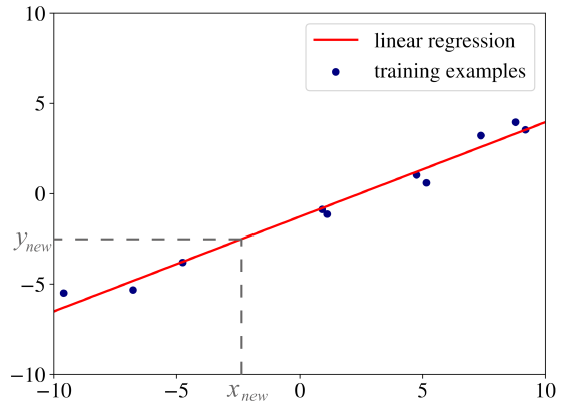
\includegraphics[width=12cm]{assets/PartOne/Chaptertwo/régressinlinéaire.png}
    \caption{Graphe représentant la régression linéaire}
    \label{régressinlinéaire}
    \end{figure}

    \newpage

\paragraph{La régression logistique :}
La régression logistique est un algorithme d'apprentissage automatique qui est utilisé pour les problèmes de classification, c'est un algorithme d'analyse prédictive basé sur le concept de probabilité. En effet, la régression logistique est un modèle linéaire généralisé qui utilise une fonction logistique comme une fonction de lien. La figure \ref{lafonctionlogistique} montre un graphe représentant la régression logistique : 

\begin{figure}[h]
    \centering
    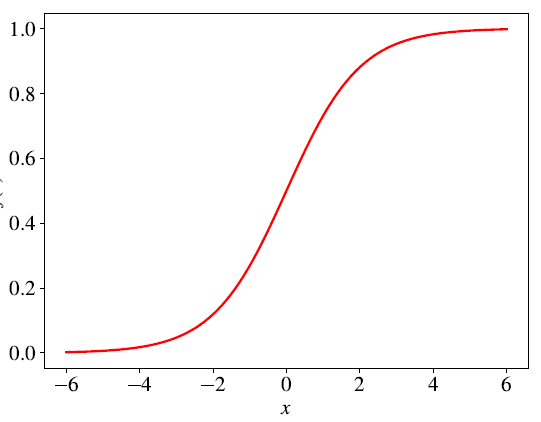
\includegraphics[width=10cm]{assets/PartOne/Chaptertwo/lafonctionlogistique.png}
    \caption{Graphe représentant la régression logistique}
    \label{lafonctionlogistique}
    \end{figure}


\paragraph{Le support vecteur machine : }
Cet algorithme utilise des hyperplans pour séparer les données. Dans le cas où cette séparation n'est pas possible, il utilise l'astuce du noyau où la dimension est augmentée et où les points de données deviennent séparables par un hyperplan \cite{RegressionAlgorithmsRegression2021}. La Figure \ref{supportvectormachine} montre un graphe représentant le support vecteur machine.


\begin{figure}[h]
    \centering
    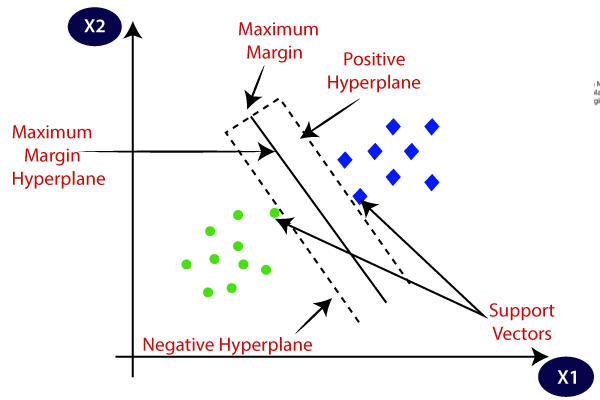
\includegraphics[width=10cm]{assets/PartOne/Chaptertwo/supportvectormachine.png}
    \caption{Graphe représentant le support vecteur machine}
    \label{supportvectormachine}
    \end{figure}

    \newpage

\paragraph{Apprentissage non supervisé}
Dans l'apprentissage non supervisé, les données d'apprentissage ne sont pas étiquetées. Le système essaie d'apprendre sans entrainement \cite{aggarwalNeuralNetworksDeep2018}. La Figure \ref{apprentissagenonsupervisé} montre exemple d’un ensemble d'entraînement non étiqueté pour l’apprentissage non supervisé.

\begin{figure}[h]
    \centering
    \includegraphics[width=10cm]{assets/PartOne/Chaptertwo/apprentissagenonsupervisé.png}
    \caption{Exemple d’un ensemble d'entraînement non étiqueté pour l’apprentissage non supervisé}
    \label{apprentissagenonsupervisé}
    \end{figure}

Ce type d’apprentissage contient aussi deux approches, le Clustering et l’Association. 

Le clustering est une méthode de regroupement des objets en clusters, de sorte que les objets présentant le plus de similitudes restent dans un groupe et ont moins ou pas de similitudes avec les objets d'un autre groupe. L'analyse par grappes trouve les points communs entre les objets de données et les catégorise en fonction de la présence ou de l'absence de ces points communs.

L’association est une méthode d'apprentissage non supervisée qui est utilisée pour trouver les relations entre les variables dans une grande base de données. Elle détermine l'ensemble des éléments qui se produisent ensemble dans l'ensemble de données. La règle d'association rend la stratégie de marketing plus efficace. Par exemple, les personnes qui achètent un article X (un pain, par exemple) ont également tendance à acheter un article Y (beurre/confiture). Un exemple typique de règle d'association est l'analyse du panier de la ménagère.

Puisque notre étude ne se concentre pas sur l'apprentissage non supervisé dans ce mémoire, on a pas détailler les algorithmes de ce type.

\paragraph{Apprentissage semi-supervisé}
L'apprentissage semi-supervisé est une classe de techniques d'apprentissage automatique qui utilise un ensemble de données étiquetées et non étiquetées. Il se situe ainsi entre l'apprentissage supervisé qui n'utilise que des données étiquetées et l'apprentissage non supervisé qui n'utilise que des données non étiquetées. Il a été démontré que l'utilisation de données non étiquetées, en combinaison avec des données étiquetées, permet d'améliorer significativement la qualité de l'apprentissage .
    
\part{Part two}
%\chapter{Cadre Méthodologique}
\section{Introduction}
La recherche scientifique est un processus nécessaire pour avoir un niveau de rigueur spécifique et assurer l'acquisition de nouvelles connaissances. Cette démarche permet d'examiner et de résoudre des circonstances et des problèmes afin d'apporter des solutions à la suite d'une enquête. 

Tout travail scientifique suit une technique de recherche qui diffère légèrement en fonction du contexte dans lequel il a été élaboré et du domaine d'application prévu.

Dans ce chapitre nous allons définir le cadre méthodologique de notre travail : Nous allons tout d’abord exposer la problématique que nous avons choisie et présenter des hypothèses en conséquence. 

Puis, nous allons expliquer l'approche de notre travail et le processus que nous avons suivi. Pour clarifier le cheminement des étapes suivies dans ce projet.  

Enfin, nous allons présenter les outils nécessaires que nous avons utilisés pour mener à bien ce projet et indiquer les spécificités des données utilisées dans ce travail.

\section{Choix du thème et problématique}
Notre projet de fin d’étude est une proposition de l'entreprise RMBtech Smart Automation, et qui a été développée tout au long de notre stage. 

La proposition est rentrée dans le cadre du thème \textbf{Contrôle de la qualité}, cette proposition répond aux besoins du cahier de charge d’un client de RMBtech. Qu’il cherche de diminuer le taux des produits non-conformes dans une ligne de production.
L’entreprise RMBtech a proposé de \textbf{\textit{développer une application pour détection de non-conformités dans une lignes de production des nouilles par le deep learning}} , ce qui est le sujet de notre projet de fin d'étude. 
\newpage
\subsection{Problématique}
A partir du deuxième chapitre de la première partie, nous disons que les applications développées par le deep learning consiste à implémenter des modèles de réseaux de neurones profonds.

Pour notre projet et comme il consiste à détecter les défauts des nouilles pour distinguer entre les conformes et les non conformes, nous avons constaté que les défauts produits dans les pièces des nouilles se retrouvent au niveau de la forme de la nouille. La figure \ref{DefautNouilles1} montre des cas de non conformités

\begin{figure}[h]
    \centering
    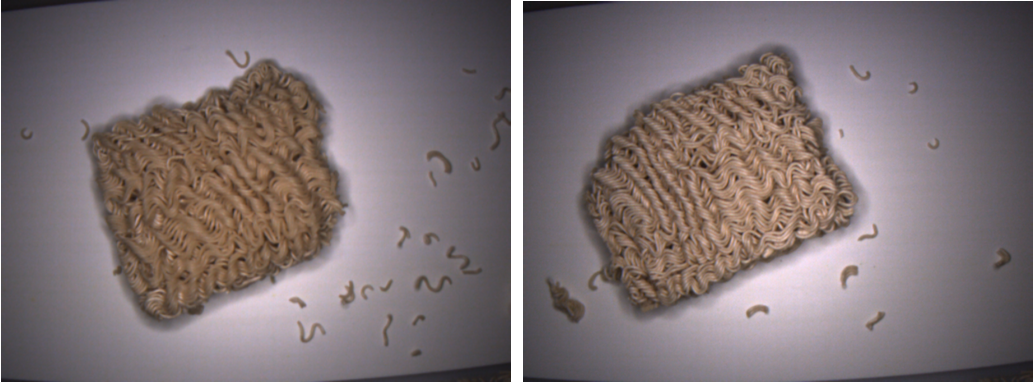
\includegraphics[width=13cm]{assets/PartTwo/Chapterone/DefautNouilles.png}
    \caption{Defaut Nouiiles}
    \label{DefautNouilles1}
    \end{figure}

Nous avons dit précédemment que les réseaux de neurones conventionnels (CNN) sont les plus utilisés pour la détection et la classification des formes et des images. 
Pour cela, notre projet de fin d’étude présenté aborde la problématique de \textbf{\textit{“Quelle est le modèle CNN le plus approprié pour une application de détection de non-conformité ?”}}
\subsection{Hypothèses}  
Suite aux recherches et à l'audition d'experts dans le domaine, les hypothèses suivantes ont été développées : 
\begin{itemize}
    \item Il est préférable d'implémenter un modèle qui avait une architecture dense qui contient plusieurs couches convolutif pour avoir une bonne précision.
    \item Il est préférable d'implémenter un modèle avec un temps d'inférence court pour détecter tous les objets passant sur le convoyeur à grande vitesse.
    \item Il est préférable d'implémenter un modèle de petite taille pour minimiser le temps d’inférence.
\end{itemize}
\newpage
\subsection{Objectif}
Le but de ce travail est de trouver le modèle le plus approprié à utiliser dans une application de détection de non-conformité sur une ligne de production de nouilles. 

Un autre objectif pour nous est de comprendre et d'appliquer les connaissances que nous avons durant notre formation à un scénario du monde réel où nous allons tester notre solution sur un cas réel, tout en utilisant une méthode scientifique. 
\section{Méthodologie du travail}
Du fait de la similarité entre les hypothèses citées ci-dessus, nous avons trouvé intéressant de regrouper les points communs entre ces dernières, qu’ils sont la précision, la taille du modèle et le temps d’inférence. 

En fait, notre travail consiste à identifier un modèle CNN avec un minimum de temps d'inférence, capable de détecter rapidement les nouilles lors de leur passage sur le convoyeur avec une grande vitesse. 

En vue de l’absence de travaux qui traitent un problème de détection similaire au nôtre, nous avons dû définir une démarche spécifique à ce projet. La démarche que nous avons suivie est le fruit de notre réflexion et de notre travail. 
\subsection{Approche}
Pour ce projet, nous avons utilisé une approche comparative qui consiste à évaluer différents modèles de CNN selon des critères précis. Ces critères sont les suivants : 
\begin{itemize}
    \item Le temps d’inférence.
    \item La précision du modèle. 
    \item La taille du modèle. 
\end{itemize}
Nous allons détailler chaque critère ci-dessous : 

\textbf{Le temps d’inférence: }Le temps d'inférence d'un modèle DNN est le temps exécuter par processus de traitement de données pour calculer une sortie telle qu'un score numérique unique. Ce processus est également appelé "mise en production d'un modèle d'apprentissage automatique". 

\textbf{La précision du modèle: }La précision est également appelée valeur prédictive positive. Elle mesure la capacité du modèle à ne pas faire d'erreur lors d'une prédiction positive. La précision est calculée à partir de la matrice de confusion avec la formule suivante : 

\begin{equation}
    P(\%)=\frac{T P+T N}{T P+T N+F P+F N} \times 100
    \end{equation}

Où P désigne la précision et TP, TN, FP, FN sont expliqué dans le chapitre trois de la premiére partie.  
\newpage
\textbf{La taille du modèle :} La taille d'un modèle DNN correspond à la quantité en mégabits (Mb) dont le modèle a besoin pour être stocké dans un environnement approprié .

Le but de ce travail est de trouvé le modèle idéal qui satisfaire les trois caractéristiques. La Figure \ref{ObjectifCible} illustre l’objectif ciblé: 

\begin{figure}[h]
    \centering
    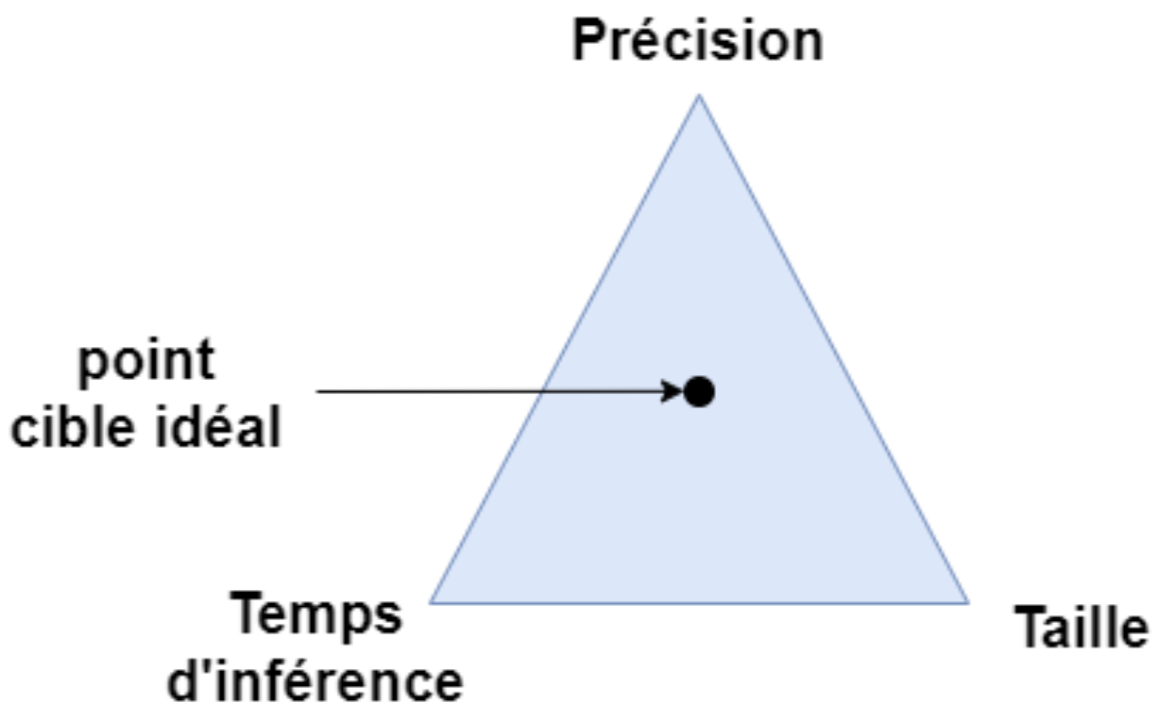
\includegraphics[width=10cm]{assets/PartTwo/Chapterone/ObjectifCible.png}
    \caption{Objectif Cible}
    \label{ObjectifCible}
    \end{figure}

\subsection{Démarche}
Notre approche commence par la collecte des données, qui sont essentiellement des images des nouilles prises par une caméra montée sur la ligne de production. 

La manière de procéder par la suite consiste à : 
\begin{itemize}
    \item Prétraiter les images collectées, afin de mieux exploiter les caractéristiques de ces images. 
    \item Préparer et classer manuellement les images en deux catégories (good / defect) , cette étape est essentielle car nous allons utiliser l'apprentissage supervisé. 
    \item Entraînement des quatre modèles avec les images prétraitées, ces modèles sont sélectionnés à partir d'une évaluation théorique basée sur les spécifications fournies dans la plateforme Keras.
    \item Évaluer chaque modèle de manière pratique sur la base des trois caractéristiques définies dans le point précédent (temps d'inférence, précision et taille du modèle).
    \item Comparer et analyser les trois modèles et sélectionner celui qui convient le mieux à notre solution. 
\end{itemize}
\newpage
Cette démarche peut être visualisée par l’organigramme présent sur la Figure %____%
\newpage
\subsection{Outils}
Plusieurs outils nous ont été utiles dans notre démarche de travail que ce soit en phase d’acquisition, de structuration, de traitement, ainsi que de visualisation des données :
\begin{itemize}
    \item Une caméra est utilisée dans notre solution pour capturer les images des nouilles, c'est une caméra à balayage de zone de marque Mindvision %ref%.
    \item Langage de programmation Python version 3.7. 
    \item La bibliothèque Keras pour utiliser ces modèles CNN.  
    \item Matplotlib pour les graphiques.
    \item Numpy pour les calculs. 
    \item OpenCV pour le traitement d'images. 
    \item Une Edge TPU (NPU) utilisé comme un ordinateur de traitement.
\end{itemize}
\bigskip
\bigskip
D’autres outils nous ont été utiles dans la rédaction du mémoire : 
\begin{itemize}
    \item Google Docs pour la rédaction. 
    \item Draw.io, Adobe Illustrator pour la réalisation des schémas et dessins graphiques. 
    \item Zotero pour la gestion des sources bibliographiques et leur citation.
\end{itemize}

\subsection{Propriété intellectuelle }
Notre travail s'est déroulé au sein d'une entreprise, le code de l'application réalisée et certaines caractéristiques des outils technologiques ne sont donc pas publiables à travers ce document. Certaines données et codes supplémentaires sont présentés en annexe. 

Les schémas et les graphiques sont réalisés par l'auteur, sauf s’ils contiennent une référence ou que le contraire soit explicité. 

\newpage
\section{Conclusion}

Dans ce chapitre, il était question de cadrer notre travail méthodologiquement. Nous avons tout d’abord déterminé les critères à prendre en compte pour notre application qui nous a permis de formuler la problématique et de proposer des hypothèses à vérifier. Par la suite, nous avons présenté notre approche inspirée de la comparaison des modèles CNN pour la classification des images %ref%  
pour traiter notre problématique. 

Enfin, nous avons présenté notre démarche sous la forme d'un organigramme, abordé le point de l'acquisition, du traitement et de la confidentialité des données, et présenté les outils que nous avons utilisés tant pour notre travail que pour ce document.

Dans le prochain chapitre, l'architecture de notre application sera expliquée. De plus, nous allons citer tout le matériel utilisé. Ensuite, on va faire une analyse comparative des modèles CNN existants afin de sélectionner les quatre meilleurs modèles. Enfin, nous allons implémenter et tester chacun de ces quatre modèles afin de sélectionner le meilleur modèle pour notre application. 
%\chapter{Etude Comparative et Choix du Modèle}
\section{Introduction}
Tout d'abord, nous allons présenter dans ce chapitre l'architecture de notre solution avec tous les composants nécessaires, puis nous allons reprendre les critères de comparaison présentés dans le cadre méthodologique. Pour évaluer les modèles CNN existants dans la bibliothèque Keras. 

Ensuite, nous allons trier ces modèles et tirer les quatre meilleurs modèles par rapport aux critères définis précédemment. Ces modèles seront implémentés dans un cas réel afin de comparer leurs performances en pratique.  

A la fin de ce chapitre, nous allons sélectionner le modèle le plus approprié pour notre application. 

\section{Architecture de la solution}
L'approche consiste à créer une application de vision artificielle capable d'utiliser une caméra de détection pour distinguer les nouilles conformes des nouilles non conformes. La caméra capture des images des nouilles pendant leur déplacement sur la ligne de production. Ces images sont capturées en temps réel à l'aide d'une photocellule qui détecte l'arrivée des nouilles et transmet des impulsions électriques à la caméra pour capturer la zone de détection. 

Les images sont envoyées à la base de données du logiciel pour être traitées en temps réel. Ce logiciel est implémenté dans un TPU qui est le cerveau de l'ensemble du système. Ce TPU dispose d'un modèle d'apprentissage profond qui peut traiter ces images et distinguer les nouilles conformes et non-conformes en fonction des caractéristiques qui ont été entraînées auparavant. Nous détaillerons la phase d'entraînement du modèle dans la suite de ce chapitre. Le modèle comprend les caractéristiques de la nouille et cela signifie que s'il y a un changement dans les caractéristiques de la nouille, il trouvera s'il s'agit d'un changement normal, donc la nouille est toujours conforme, ou d'un changement anormal, donc la nouille est non conforme. 
\newpage
Suite à la réponse du modèle, autrement dit l'inférence, le TPU délivre un signal au vérin à l'aide de broches d'entrée/sortie. Si la nouille est conforme, le vérin réagit en fonction de l'inférence et la laisse passer. Si elle n'est pas conforme, elle sera poussée hors du convoyeur et placée dans un sac spécial pour les nouilles non conformes .la figure ci-dessous représente un schéma explicatif sur la solution complète : 

\begin{figure}[h]
    \centering
    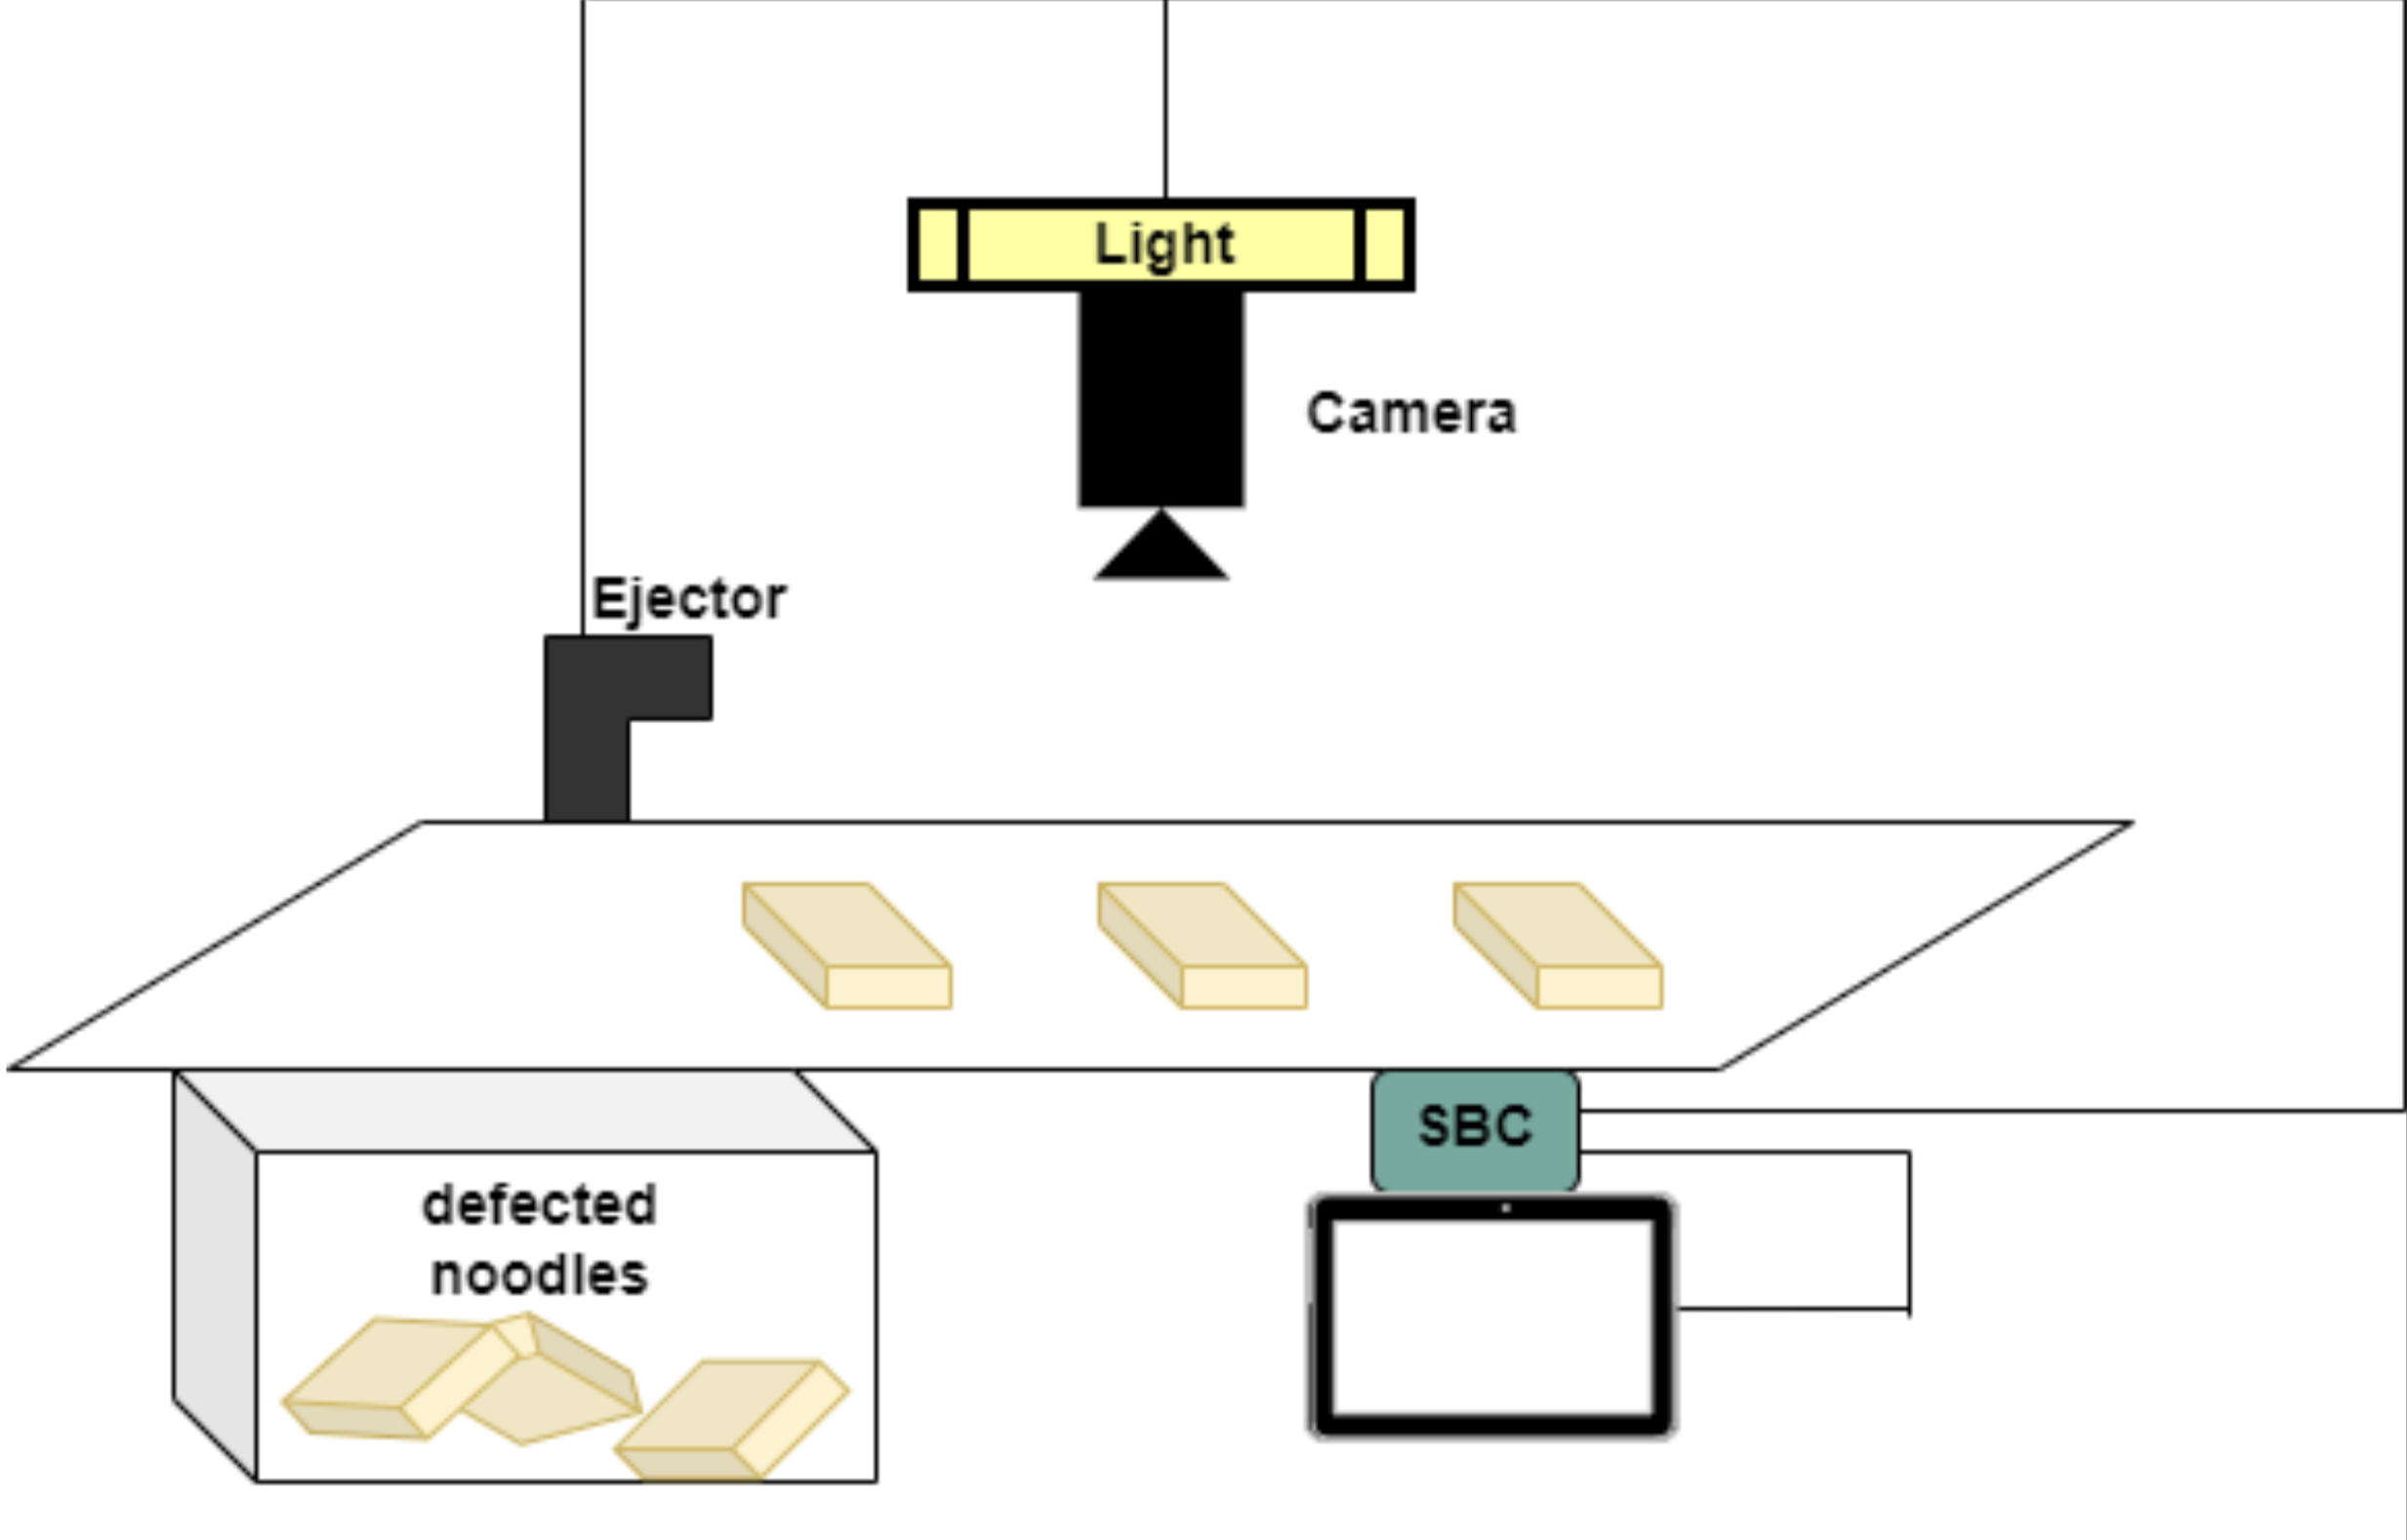
\includegraphics[width=10cm]{assets/PartTwo/Chapterone/ShemaExplicatif.png}
    \caption{Schema explicatiof}
    \label{SchemaArchitecture}
    \end{figure}

Pour faciliter le travail, le logiciel devra être commandé par une interface utilisateur graphique (GUI) moderne et simple, l'interface est représentée sur un écran tactile pour permettre à l'opérateur de contrôler le système, de le configurer, d'extraire les résultats et de voir les statistiques en temps réel .la figure suivante représente GUI de notre système :
GuiInterface 
\begin{figure}[h]
    \centering
    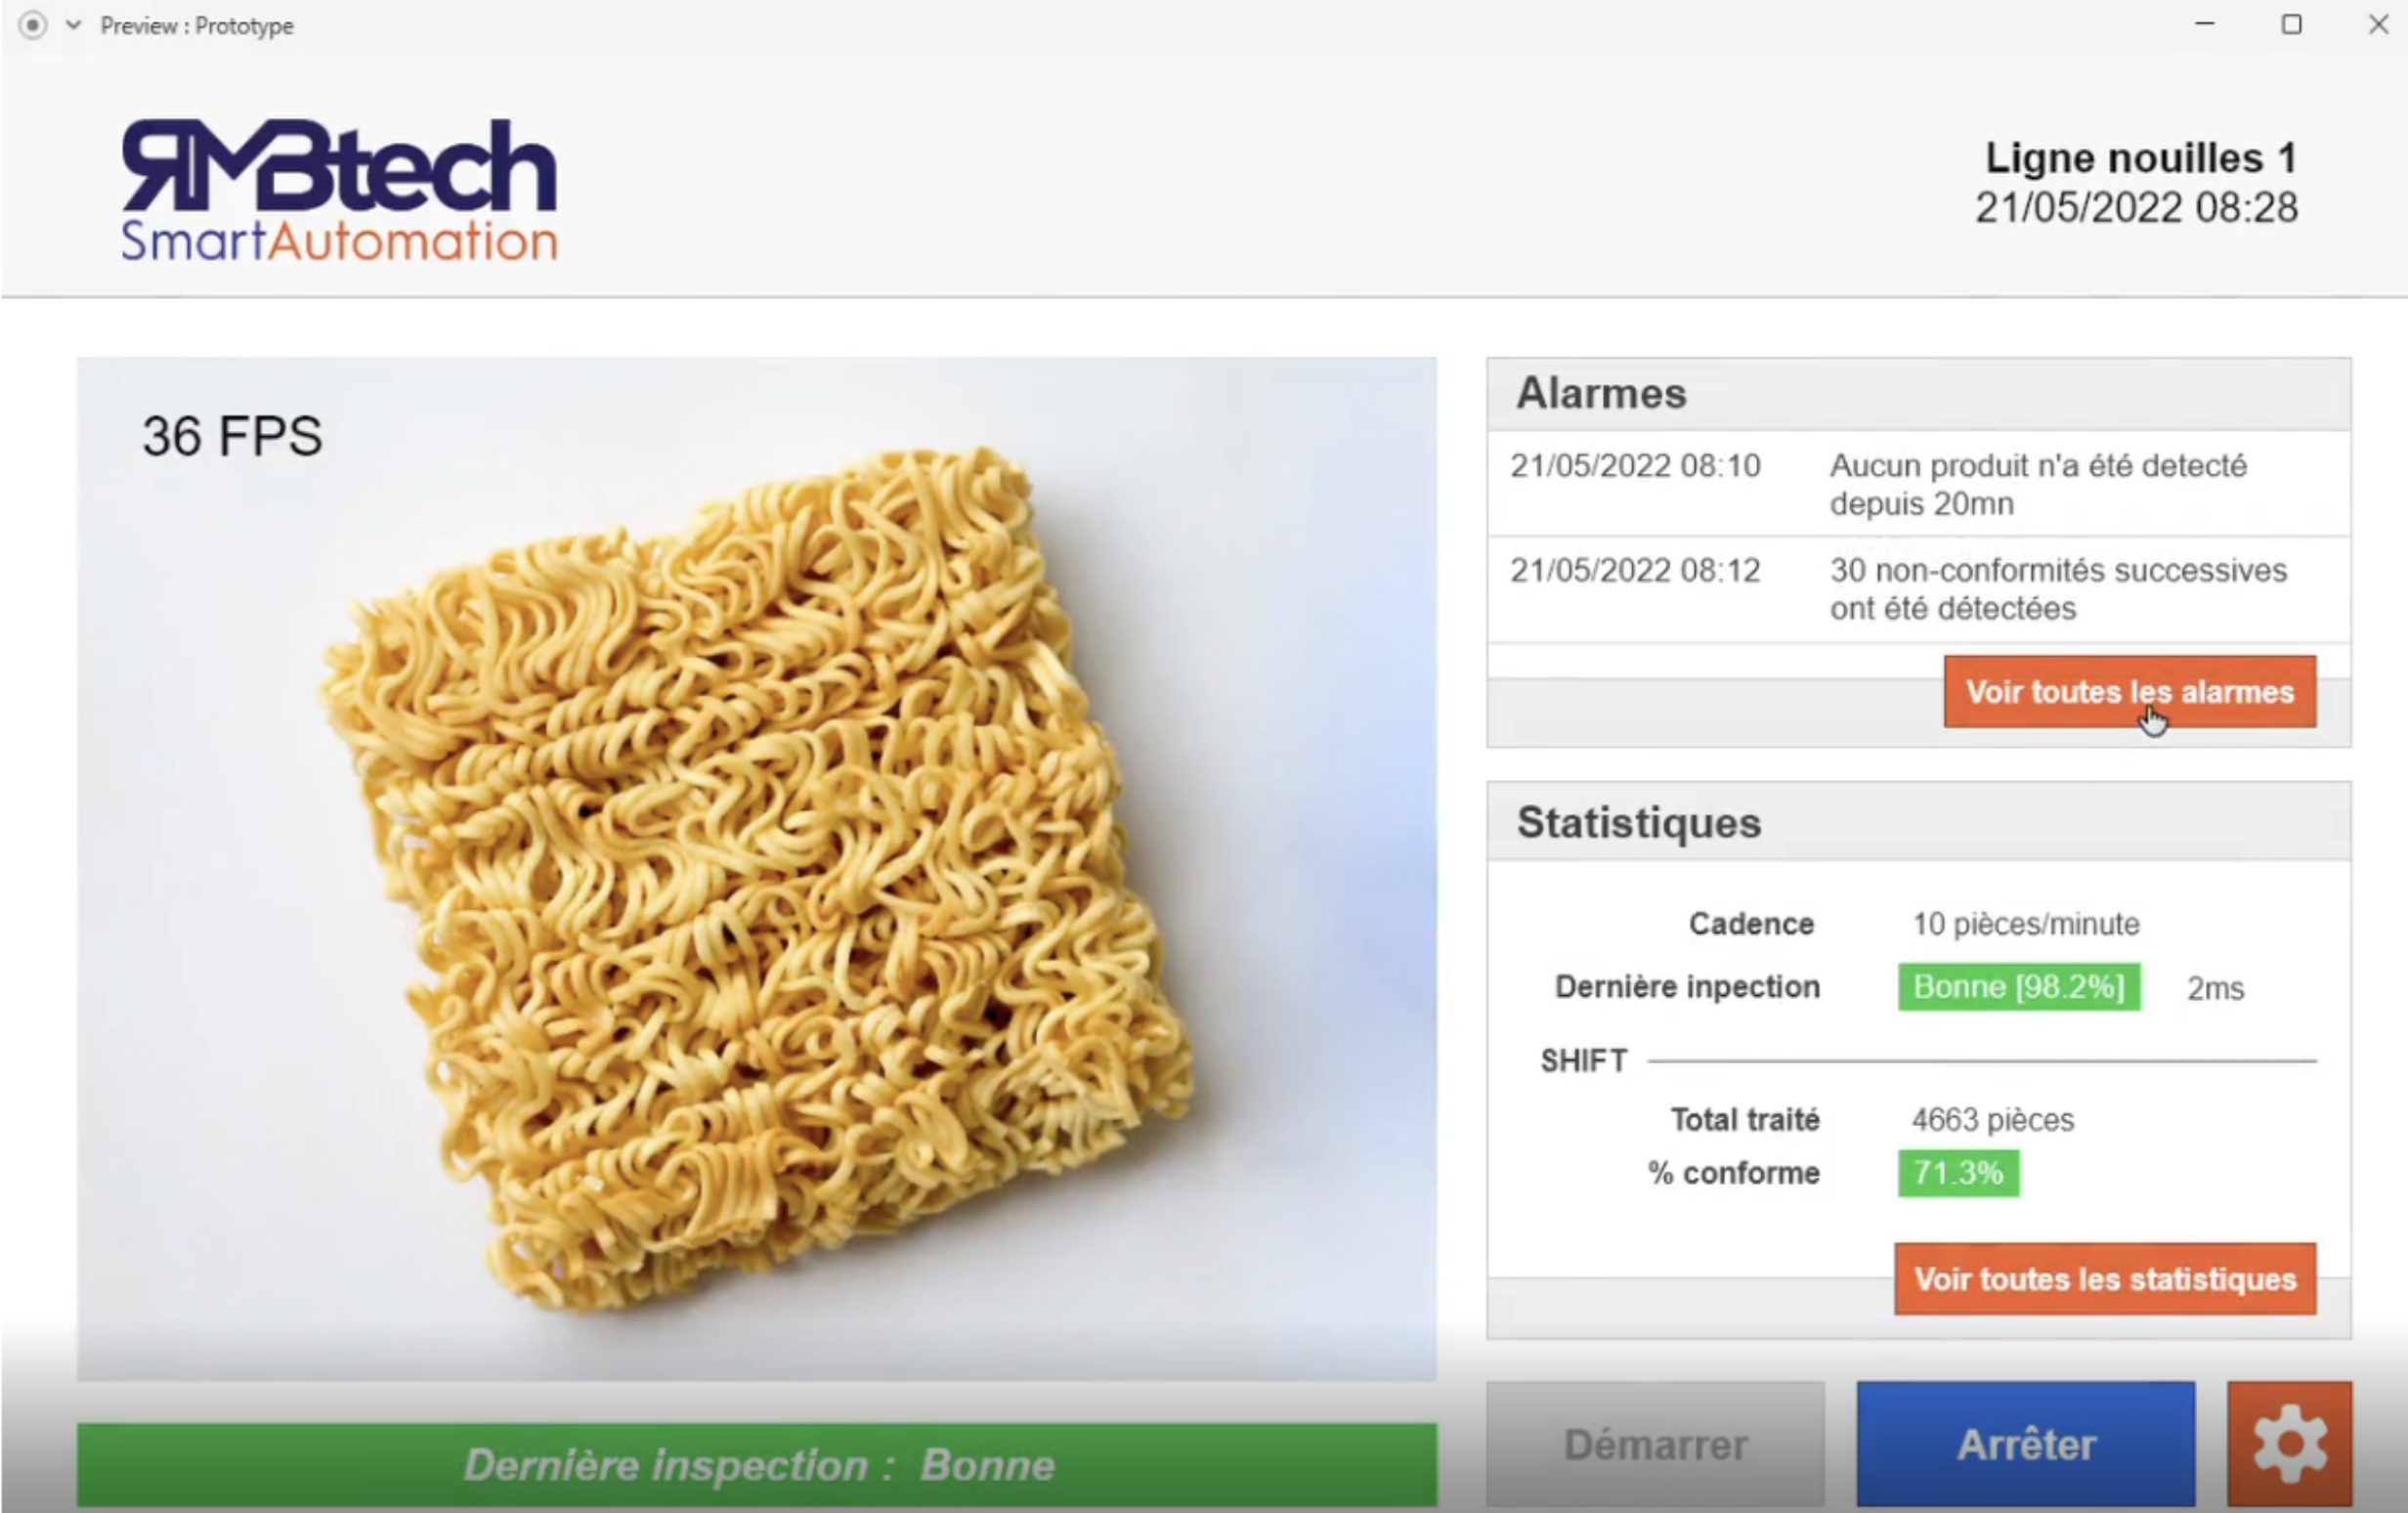
\includegraphics[width=12cm]{assets/PartTwo/ChapterTwo/GuiInterface.png}
    \caption{GUI}
    \label{GUI}
    \end{figure}

\newpage
\section{Configuration Hardware et Software}
Dans ce point, nous allons décrire les choix techniques de l'ensemble de la partie matérielle (Hardware) et partie logiciel (Software). 
\subsection{Choix de la caméra : }
Nous avons choisi une caméra à zone de balayage car elle nous permet de recevoir rapidement une image de la zone des nouilles, et dans le cas d'un contrôle de non-conformité en temps réel, la vitesse du système est un facteur critique. Pour des raisons de rapidité également nous avons fixé la résolution à 800*600 et cela augmentera les FPS c'est-à-dire augmentera la vitesse de capture de la caméra. Lorsque la nouille traverse le champ de la photocellule l'image est capturée. Dont le champ de détection de la photocellule est de 6 cm. 
\subsection{Choix d'éclairage : }
Nous avons utilisé un éclairage frontal avec une ampoule LED circulaire pour diriger la lumière vers les nouilles et éliminer les régions secondaires pour garder un focus et un contraste total sur la zone de détection de la nouille. 
\subsection{Choix du TPU : }
Nous avons utilisé le TPU Asus Tinker Edge T qui est utile pour les applications industrielles car il a une capacité de traitement élevée. Tous ces composants sont rassemblés dans un support métallique qui est installé sur une bande transporteuse et sont alimentés par une source de tension de 24V.  

\section{Préparation des données }
Notre recherche vise à catégoriser l'image des nouilles. L'ensemble de données d'entraînement et de test ont été créés à partir de l'ensemble de données original. Un ensemble de données contenant 4000 images a été utilisé dans ce travail pour l'entrainement, devisé en deux classe GOOD et DEFECT chaque classe contient 2000 images pour la validation on a pris 1000 images. Les images ont été choisies au hasard.  

L'image originale de l'appareil photo a une taille de 800 x 600 pixels. Le centre de l'image est l'endroit où se trouvent les nouilles. Les images ont été réduites à 224 x 224 pixels afin de réduire la complexité du traitement et d'être compatibles avec l'entrée du modèle. 

\newpage
La figue \ref{GoodDefectNoodles} montre un échantillon des données avec ces deux classes GOOD et DEFECT 
\begin{figure}[h]
    \centering
    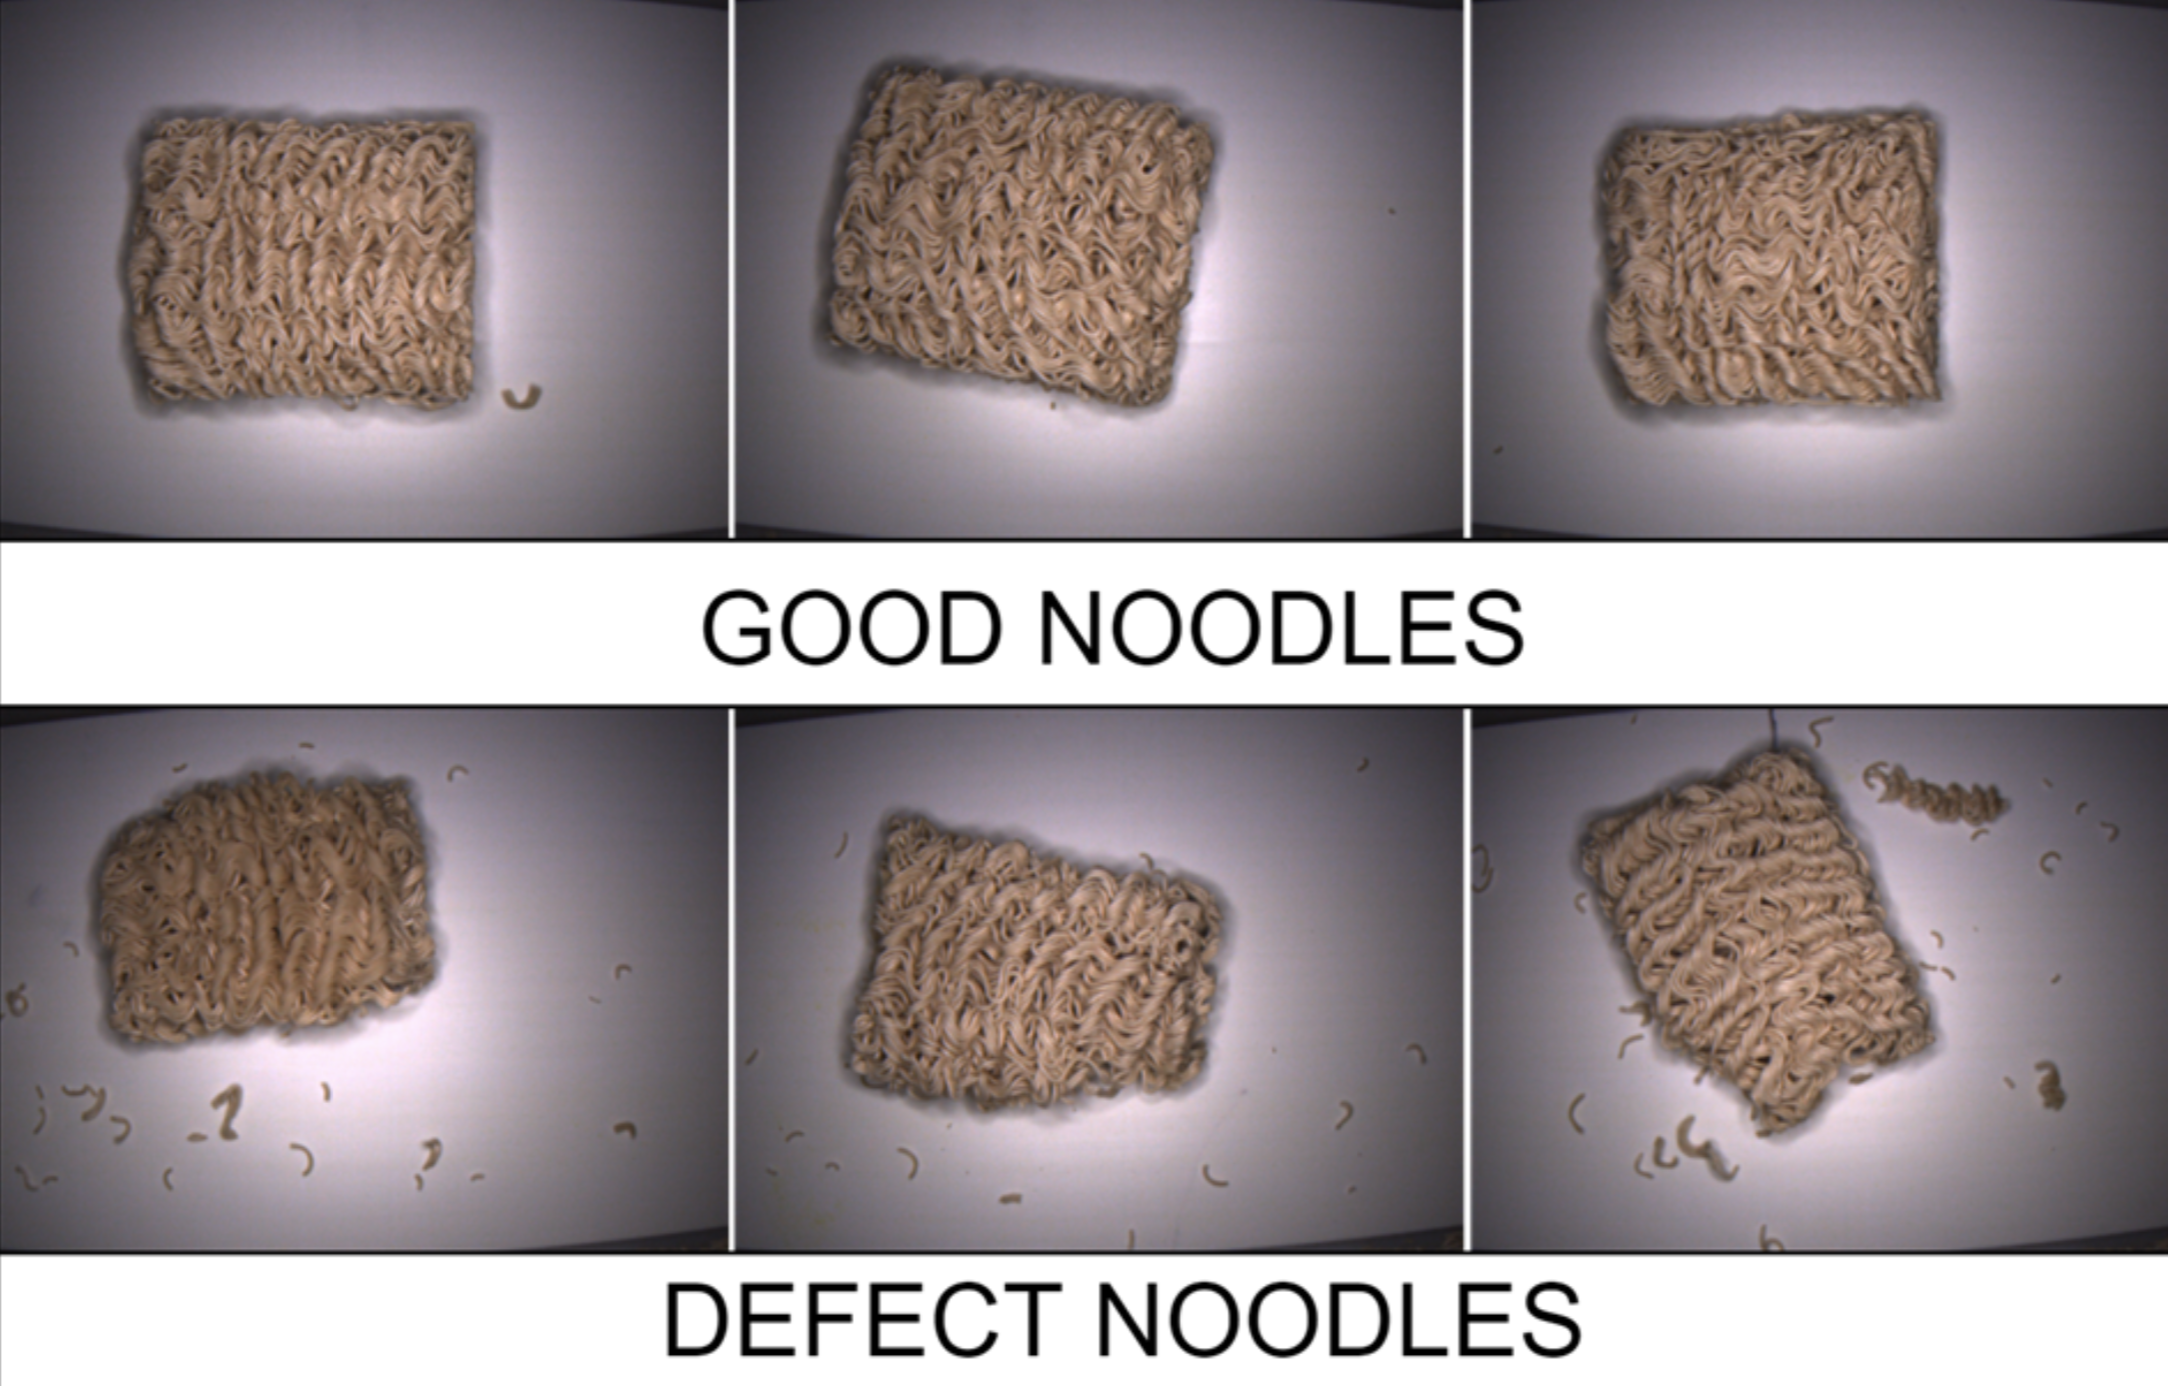
\includegraphics[width=14cm]{assets/PartTwo/ChapterTwo/GoodDefectNoodles.png}
    \caption{GoodDefectNoodles}
    \label{GoodDefectNoodles}
    \end{figure}

\section{Implémentation des modèles}
Notre travail consiste à utiliser des modèles pré-entraînés de Keras et nous allons les réentraîner avec nos données. Cette technique est appelée transfert learning, et nous l'avons abordée plus en détail dans le chapitre deux de la première partie.  
Une première sélection théorique a été faite manuellement à travers une comparaison des trois critères sur tous les modèles de Keras.  

Cette comparaison théorique a été faite à l'aide d'une matrice de décision où nous avons donné à chaque critère une note sur 10, nous n'avons pas utilisé de pondération car les trois critères ont la même importance. Le Tableau ci-dessous montre le tableau de comparaison des modèles. 
\newpage
\begin{figure}[h]
    \centering
    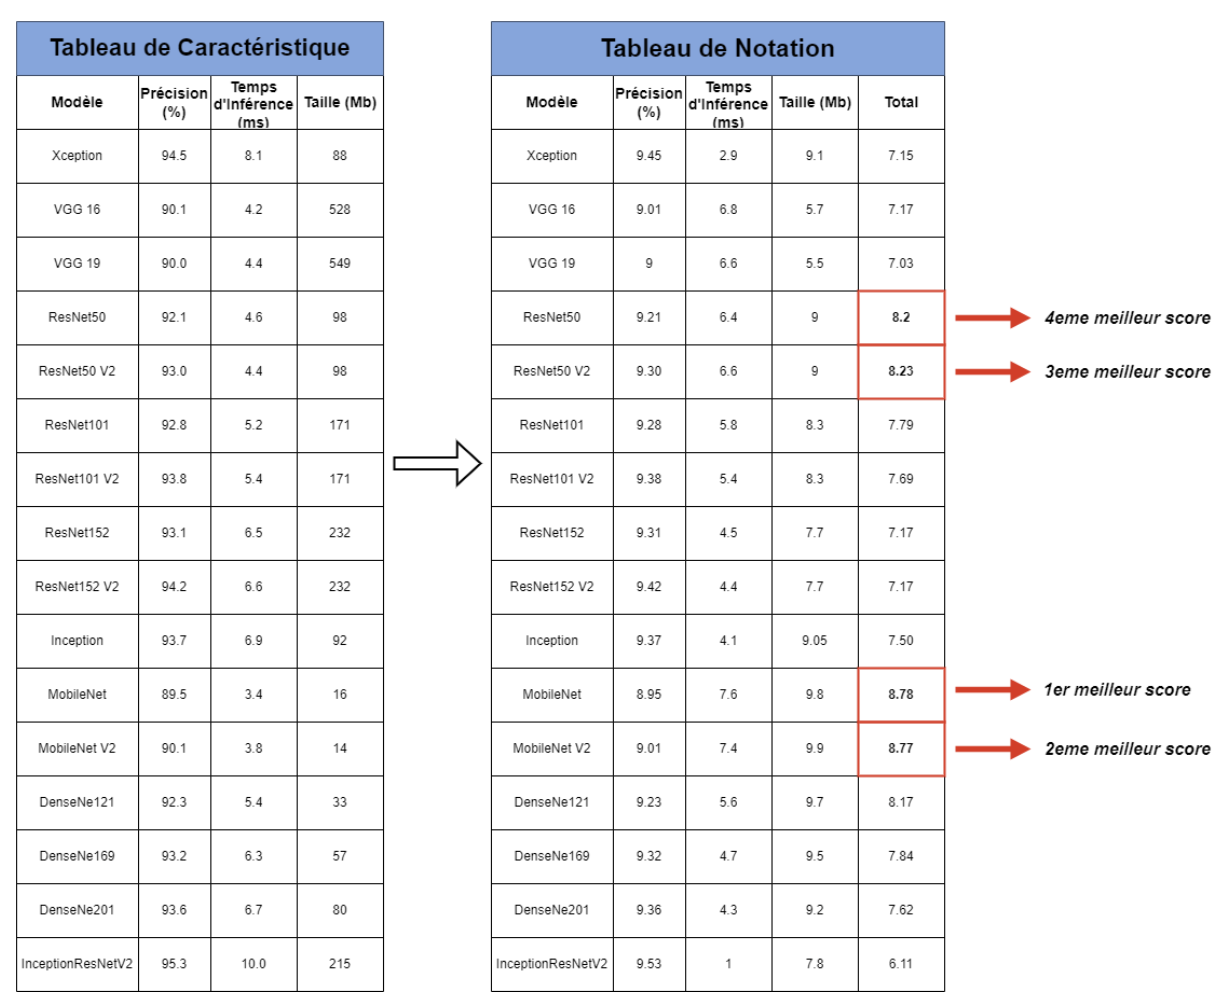
\includegraphics[width=14cm]{assets/PartTwo/ChapterTwo/ComparaisonModeles.png}
    \caption{ComparaisonModeles}
    \label{ComparaisonModeles}
    \end{figure}

    D'après la figure, nous pouvons voir que quatre modèles ont été sélectionnés et qu'ils sont les suivants : MobileNet, MobileNet V2, ResNet50, ResNet50 V2.

    Les architectures de ces modèles ont été détaillé dans le chapitre deux de la première partie. 

\section{Evaluation des modèles}
Dans cette section, nous présenterons une évaluation des caractéristiques utilisées pour comparer les performances des quatre modèles, ainsi que les résultats produits et une discussion des résultats des modèles décrits. 

Tous les modèles de cette section ont été créés avec des hyperparamètres distincts. Ces derniers ont été choisis après de multiples itérations, et pour chaque modèle, nous avons pris les hyperparamètres qui ont donné les meilleurs résultats. 


Les détails des résultats pour chaque modèle est présenté ci-dessous : 
\newpage
\subsection{MobileNet V1 }
Concernant le MobileNet, nous avons utilisé les hyperparamètres détaillés dans le tableau suivant : 

    \begin{table}[h]
        \begin{center}
            \begin{tabular}{|l|l|l|l|}
                \hline
                Forme de l'entrée & Taille du lot & Epoques & Taux d'apprentissage \\ \hline
                (224, 224)        & 32            & 500     & 5e-5                 \\ \hline
                \end{tabular}
        \end{center}
        
        \end{table}
        Le modèle atteint une précision de 99.25\% à l'entraînement et 98.21\% en teste, le taux d’erreur pour l'entraînement et le teste est respectivement 1.17\%, 8.37\%. Ce qui montre un bon résultat vu que l’erreur ne dépasse pas 10\%. Les résultats de l'entraînement et des tests de ce modèle sont présentés dans la Figure \ref{MobileNetV1Result}. 
 \begin{figure}[h]
\centering
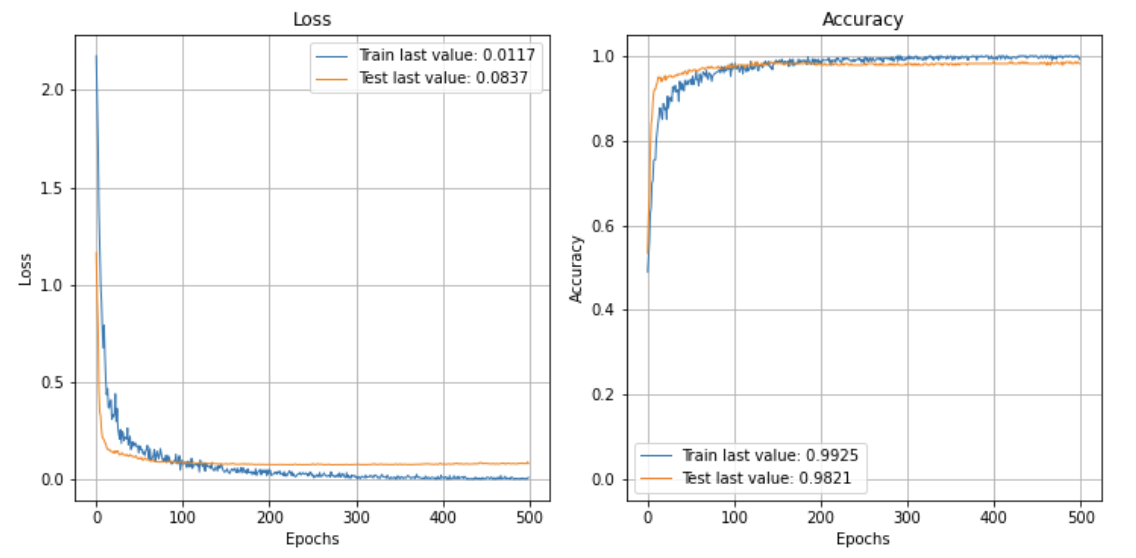
\includegraphics[width=13cm]{assets/PartTwo/ChapterTwo/MobileNetV1Result.png}
\caption{MobileNetV1Result}
\label{MobileNetV1Result}
\end{figure}

Lors de l'implémentation du modèle, nous avons trouvé les résultats suivants : la taille et le temps d'inférence pratique sont respectivement de 9,4 Mo et 3,07 ms, en ce qui concerne la précision pratique (validation), nous avons trouvé la matrice de confusion présentée dans la Figure \ref{MOBILENETV1TFTV} qui donne une précision de 96,35\%. 

\begin{figure}[h]
    \centering
    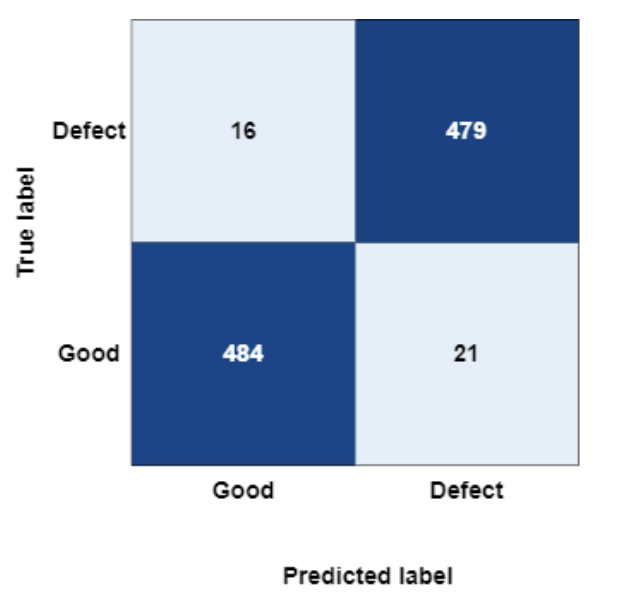
\includegraphics[width=5cm]{assets/PartTwo/ChapterTwo/MOBILENETV1TFTV.png}
    \caption{MOBILENETV1TFTV}
    \label{MOBILENETV1TFTV}
    \end{figure}
\newpage
\subsection{MobileNet V2}
Le MobileNet V2 a été entraîné avec les mêmes hyperparamètres sauf qu’on a changé le taux d’apprentissage à 1e-7. Le Tableau suivant montre les hyperparamètres d'entraînement du MobileNet V2. 
\begin{table}[h]
    \begin{center}
        \begin{tabular}{|l|l|l|l|}
            \hline
            Forme de l'entrée & Taille du lot & Epoques & Taux d'apprentissage \\ \hline
            (224, 224)        & 32            & 500     & 1e-7                 \\ \hline
            \end{tabular}
    \end{center}
    
    \end{table}
    Ce modèle a également obtenu de bons résultats en termes de précision et d'erreur. Il a atteint une précision à l'entraînement et au test de 99,75\% et 97,85\%, respectivement, l'erreur n'a pas dépassé 10\% et s'est située entre 1,21\% à l'entraînement et 7,73\% au test. La Figure \ref{MobileNetV2Result} montre les résultats d'entraînement et de test de ce modèle. 
    \begin{figure}[h]
        \centering
        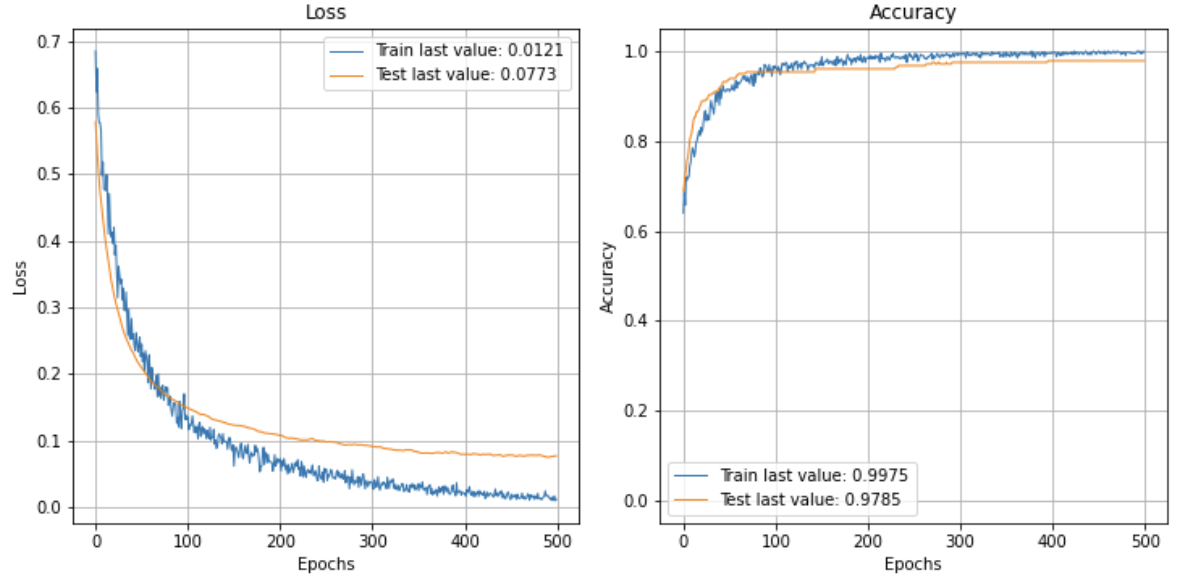
\includegraphics[width=13cm]{assets/PartTwo/ChapterTwo/MobileNetV2Result.png}
        \caption{MobileNetV2Result}
        \label{MobileNetV2Result}
        \end{figure}

La taille du modèle après implémentation est de 37,7 Mo, le temps d'inférence est de 3,9 ms et la précision de validation est de 95,9\% après le calcul de la matrice de confusion présentée à la figure \ref{MobileNetV2TFTN}.

\begin{figure}[h]
    \centering
    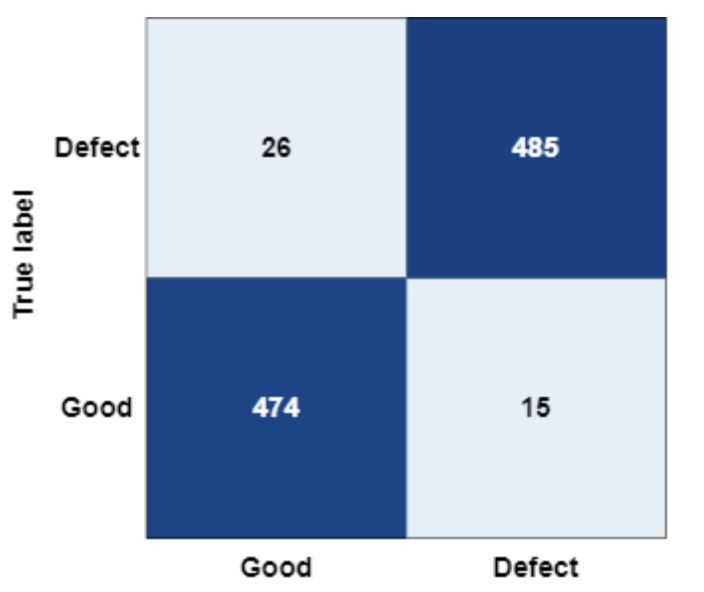
\includegraphics[width=6cm]{assets/PartTwo/ChapterTwo/MobileNetV2TFTN.png}
    \caption{MobileNetV2TFTN}
    \label{MobileNetV2TFTN}
    \end{figure}
\newpage
\subsection{ResNet50 V1 }
Pour ResNet50 V1, nous avons changé le taux d'apprentissage à 1e-5 et la taille du lot à 16. Ces hyperparamètres ont montré les meilleurs résultats pour les itérations de ResNet50 V1 et ont été représentés dans le tableau  suivant : 

\begin{table}[h]
    \begin{center}
        \begin{tabular}{|l|l|l|l|}
            \hline
            Forme de l'entrée & Taille du lot & Epoques & Taux d'apprentissage \\ \hline
            (224, 224)        & 16            & 500     & 1e-5                 \\ \hline
            \end{tabular}
    \end{center}
    \end{table}
    La précision de ce modèle était excellente, puisqu'elle était de 100\% pendant la formation et de 97,13\% pendant le test. Cependant, lorsque nous regardons l'erreur, nous observons que le modèle a plus de 14\% pour le test, ce qui indique un Overfitting donc le modèle n'est pas fiable en termes de précision. La Figure 2-6a montre les résultats de ResNet50 V1. 

    \begin{figure}[h]
        \centering
        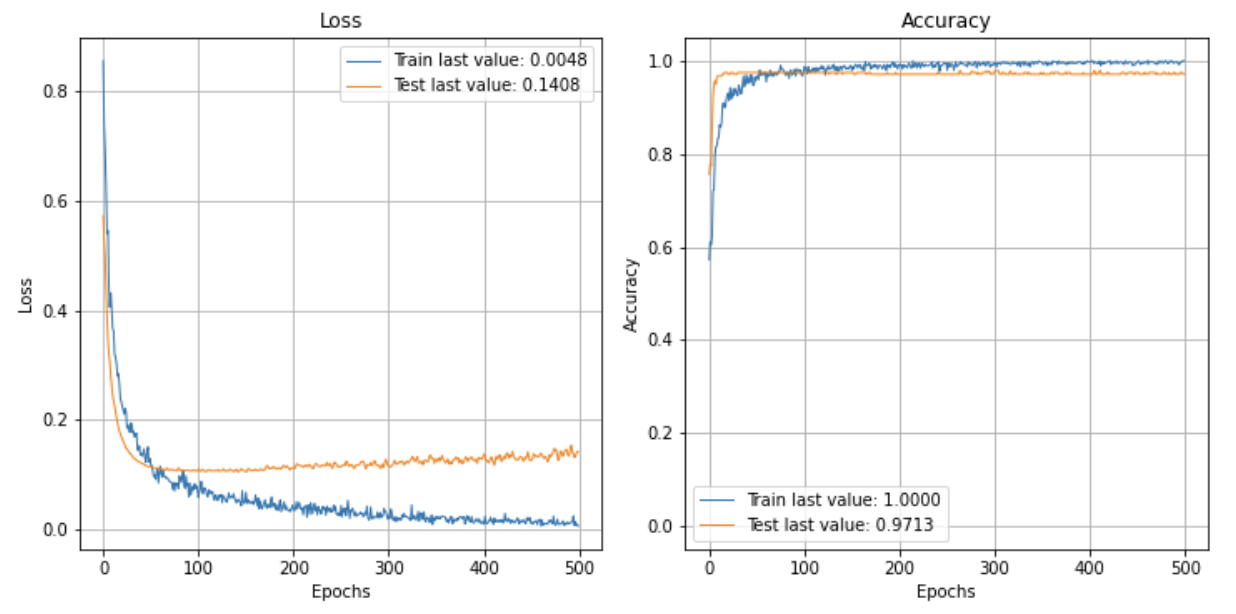
\includegraphics[width=13cm]{assets/PartTwo/ChapterTwo/ResNet50Results.png}
        \caption{ResNet50Results}
        \label{ResNet50Results}
        \end{figure}

Le modèle pratique a une taille de 103,2 Mo, avec un temps d'inférence de 5,1 ms. La précision pratique est de 88,1\%, et les propriétés de cette précision sont illustrées à la figure 2-6b. 
\begin{figure}[h]
    \centering
    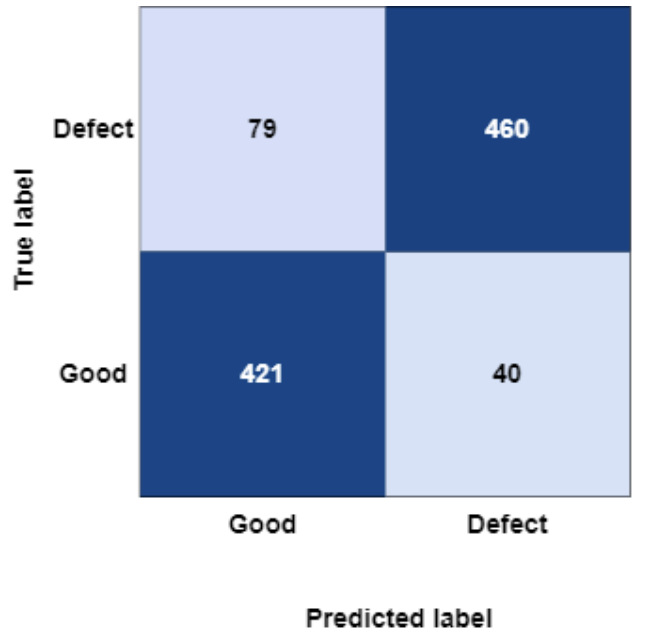
\includegraphics[width=5cm]{assets/PartTwo/ChapterTwo/ResNet50TFTN.png}
    \caption{ResNet50TFTN}
    \label{ResNet50TFTN}
    \end{figure}
\newpage

\subsection{ResNet50 V2 }
Enfin, pour ResNet50 V2, nous avons laissé la taille du lot à 32 et modifié le taux d'apprentissage à 2e-7. Le Tableau 2-5 suivant montre les hyperparamètres d'entraînement du ResNet50 V2. 
\begin{table}[h]
    \begin{center}
        \begin{tabular}{|l|l|l|l|}
            \hline
            Forme de l'entrée & Taille du lot & Epoques & Taux d'apprentissage \\ \hline
            (224, 224)        & 32            & 500     & 2e-7                  \\ \hline
            \end{tabular}
    \end{center}
    \end{table}
    Avec ces hyperparamètres, le modèle a atteint 99,5\% en entraînement et 98.21\% en test. Le modèle a atteint 1,43\% pendant l'entraînement et 6,34\% pendant les tests. La Figure \ref{ResNet50V2RESULT} montre les résultats d'entraînement et de test de ce modèle.
    \begin{figure}[h]
        \centering
        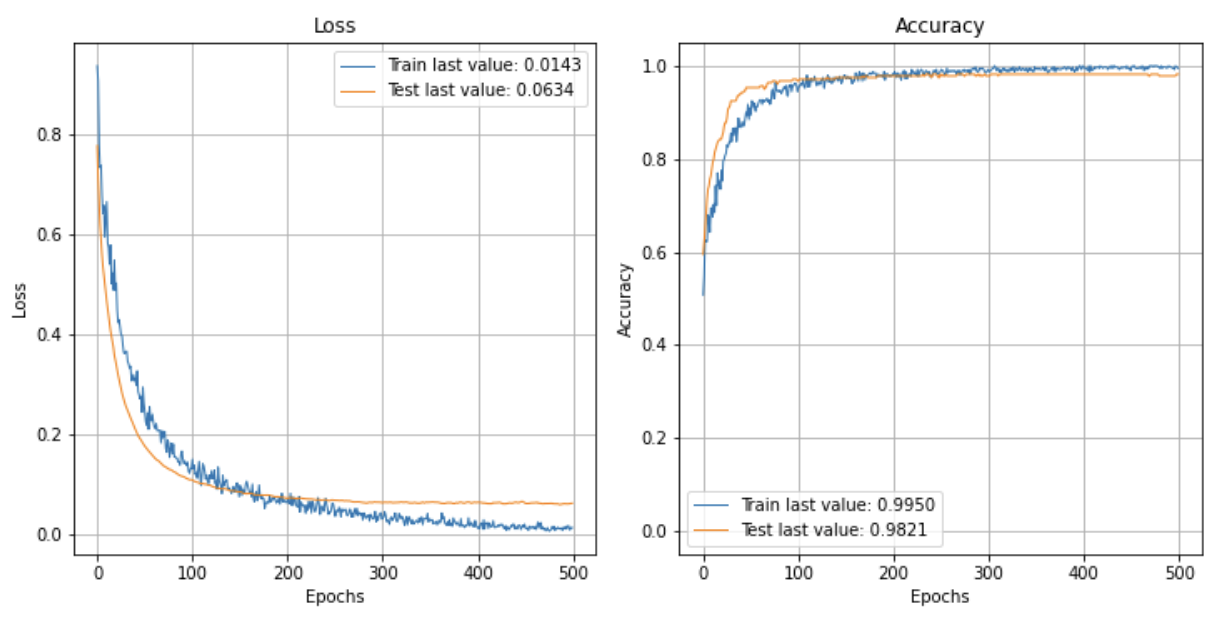
\includegraphics[width=13cm]{assets/PartTwo/ChapterTwo/ResNetV2RESULT.png}
        \caption{ResNetV2RESULT}
        \label{ResNet50V2RESULT}
        \end{figure} 
        La matrice de confusion présenté dans la Figure \ref{ResnetV2TFTD} a donné une précision pratique de 93,3\%. La taille de l'implémentation du modèle est de 322,8 Mo, et le temps d'inférence est de 9,3 ms. 

    \begin{figure}[h]
            \centering
            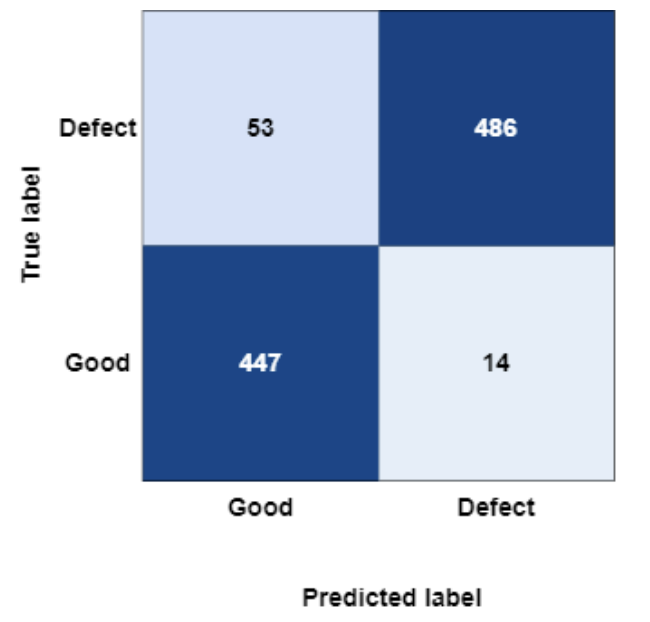
\includegraphics[width=5cm]{assets/PartTwo/ChapterTwo/ResnetV2TFTD.png}
            \caption{ResnetV2TFTD}
            \label{ResnetV2TFTD}
            \end{figure}
        \newpage
\section{Analyses et discussion des résultats}
Les résultats ci-dessus expliquent l'évaluation de chaque modèle. Comme une analyse à partir de ces résultats, nous pouvons effectuer une comparaison entre les quatre modèles en fonction des caractéristiques définies précédemment :la précision, le temps d'inférence, et la taille du modèle. 

Cette comparaison implique l'exécution d'une autre matrice de décision, similaire à celle présentée dans le tableau \ref{ComparaisonModeles}, afin d'évaluer les différences entre les caractéristique pratique de chaque modèle et de sélectionner le meilleur modèle à appliquer dans notre système. La figure suivante montre la comparaison entre les quatre modèles : 
\begin{figure}[h]
    \centering
    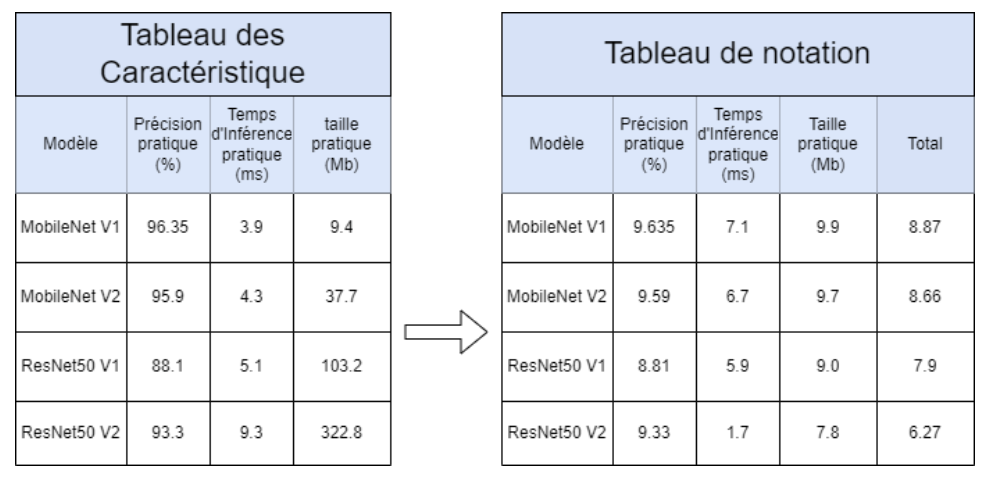
\includegraphics[width=13cm]{assets/PartTwo/ChapterTwo/TableauAnalyse.png}
    \caption{TableauAnalyse}
    \label{TableauAnalyse}
    \end{figure} 

    D'après la Figure \ref{TableauAnalyse}. Nous pouvons voir que les modèles MobileNet-V1 et MobileNet-V2 sont légèrement plus précis que le modèle Resnet50 V2. D'autre part, ResNet50-V1 est loin de cette comparaison car il a eu un effet d'overffiting qui montre une diminution de sa précision. Cela implique que l’hypothèse 1 est infirmée. 

    MobileNet-V1 est plus performant que les autres modèles en termes de temps d'inférence, car ses couches sont moins denses. Le MobileNet V2 est un peu proche au mobileNet V1 car il est aussi n’est pas dense en termes de couches convolutive. Le ResNet V1 et V2 malgré qu’ils ne soient pas dépasser les 10s mais ils ont toujours un peu lents par rapport de MobileNet V1. Donc l’hypothèse 2 est confirmée. 
    Les tailles des quatre modèles ont été modifiées car la méthode de transfert learning décrite précédemment dans le chapitre deux de la première partie implique l'ajout d'un nouveau classificateur (couches entièrement connectées) au modèle. 
    
    La taille augmentera donc proportionnellement à la taille du nouveau classificateur, mais même dans ce cas, la taille de MobileNet-V1 reste la plus petite par rapport aux autres modèles. Ceci implique que l'hypothèse 3 est infirmée car la taille du modèle à l'implémentation dépend du nouveau classificateur ajouté. 
    
    \newpage
    \section{Conclusion}
    Les trois hypothèses ont été traitées dans ce dernier chapitre par évalué chaque modèle selon les trois facteurs : la précision, le temps d'inférence et la taille du modèle. Grâce à l'application des modèles dans un cas réel. 

Ensuite, nous avons cité les hypothèses qui ont été réfutées et l'hypothèse unique qui a été confirmée. Enfin et après avoir considéré plusieurs itérations, nous avons finalement opté pour le modèle “MobileNet V1” en raison de ses performances d'implémentation. 

Ce modèle sera implémenté dans une solution complète de détection des nouilles non conforme. 


\newpage
\input{Parts/conclusion.tex}
\bibliography{bib.bib}
\bibliographystyle{plain}
\input{Parts/resume.tex}
\printglossaries
\end{document}